% !TEX program = xelatex
% Biên dịch:  latexmk -xelatex main.tex   (hoặc: xelatex → biber → xelatex → xelatex)
\documentclass[12pt,a4paper,oneside]{report}
\usepackage[fontsize=13pt]{scrextend}

% ───────── Phông chữ & ngôn ngữ ─────────
\usepackage{fontspec}
\usepackage{amsmath,amssymb,mathtools,bm}
\usepackage{unicode-math}
\setmainfont{TeX Gyre Termes}
\setmathfont{TeX Gyre Termes Math}
\setmonofont[Scale=0.85]{DejaVu Sans Mono}

% ───────── Bố cục trang ─────────
\usepackage[left=3.5cm,right=2cm,top=3cm,bottom=3cm]{geometry}
\usepackage{setspace}\onehalfspacing
\usepackage{indentfirst}\setlength{\parindent}{1cm}
\usepackage{microtype}
\emergencystretch=2em
\raggedbottom

% ───────── Gói tiện ích ─────────
\usepackage{graphicx}\graphicspath{{figures/}}
\usepackage{booktabs,multirow,array,tabularx,longtable}
\usepackage[table]{xcolor}
\usepackage{enumitem}\setlist{nosep,leftmargin=1.6cm}
\usepackage{tikz}\usetikzlibrary{arrows.meta,positioning,calc,fit,backgrounds}
\usepackage[font=small,labelfont=bf,labelsep=period,skip=6pt]{caption}
\usepackage{subcaption}
\usepackage{adjustbox}
\usepackage{algorithm}
\usepackage[noend]{algpseudocode}
\usepackage{csquotes}
\usepackage[backend=biber,style=numeric-comp,sorting=nyt,maxbibnames=6,minbibnames=3,giveninits=true,doi=true,url=false,isbn=false,eprint=true]{biblatex}
\addbibresource{references.bib}
\usepackage[hidelinks,unicode]{hyperref}

% ───────── Tên gọi tiếng Việt ─────────
\renewcommand{\contentsname}{MỤC LỤC}
\renewcommand{\listfigurename}{DANH MỤC HÌNH VẼ}
\renewcommand{\listtablename}{DANH MỤC BẢNG BIỂU}
\renewcommand{\figurename}{Hình}
\renewcommand{\tablename}{Bảng}
\renewcommand{\chaptername}{CHƯƠNG}
\renewcommand{\appendixname}{PHỤ LỤC}
\floatname{algorithm}{Thuật toán}
\renewcommand{\algorithmicrequire}{\textbf{Đầu vào:}}
\renewcommand{\algorithmicensure}{\textbf{Đầu ra:}}
\DefineBibliographyStrings{english}{andothers={và cộng sự},and={và},pages={tr\adddot},page={tr\adddot},in={Trong},techreport={Báo cáo kỹ thuật},phdthesis={Luận án tiến sĩ},edition={ấn bản},volume={tập},number={số}}
\defbibheading{bibliography}[TÀI LIỆU THAM KHẢO]{\chapter*{#1}\addcontentsline{toc}{chapter}{#1}}

% ───────── Định dạng tiêu đề ─────────
\usepackage{titlesec}
\titleformat{\chapter}[display]{\normalfont\bfseries\centering\large}{\MakeUppercase{\chaptertitlename} \thechapter}{4pt}{\Large\MakeUppercase}
\titleformat{name=\chapter,numberless}[block]{\normalfont\bfseries\centering\Large}{}{0pt}{}
\titlespacing*{\chapter}{0pt}{-10pt}{24pt}
\renewcommand{\thesection}{\thechapter.\arabic{section}}
\titleformat{\section}{\normalfont\bfseries\large}{\thesection.}{0.5em}{}
\titleformat{\subsection}{\normalfont\bfseries\itshape}{\thesubsection.}{0.5em}{}
\titleformat{\subsubsection}{\normalfont\itshape}{}{0em}{}
\titlespacing*{\section}{0pt}{14pt}{6pt}
\titlespacing*{\subsection}{0pt}{10pt}{4pt}
\setcounter{secnumdepth}{2}\setcounter{tocdepth}{2}

\usepackage{tocloft}
\renewcommand{\cfttoctitlefont}{\hfill\bfseries\Large}\renewcommand{\cftaftertoctitle}{\hfill}
\renewcommand{\cftloftitlefont}{\hfill\bfseries\Large}\renewcommand{\cftafterloftitle}{\hfill}
\renewcommand{\cftlottitlefont}{\hfill\bfseries\Large}\renewcommand{\cftafterlottitle}{\hfill}
\renewcommand{\cftchapfont}{\normalfont}\renewcommand{\cftchappagefont}{\normalfont}
\renewcommand{\cftchapleader}{\cftdotfill{\cftdotsep}}
\renewcommand{\cftchappresnum}{CHƯƠNG }\renewcommand{\cftchapaftersnum}{.}
\setlength{\cftchapnumwidth}{2.6cm}\setlength{\cftbeforechapskip}{2pt}
\setlength{\cftsecindent}{0.8cm}\setlength{\cftsubsecindent}{1.9cm}
\renewcommand{\cftfigpresnum}{Hình }\setlength{\cftfignumwidth}{1.9cm}\setlength{\cftfigindent}{0pt}
\renewcommand{\cfttabpresnum}{Bảng }\setlength{\cfttabnumwidth}{1.9cm}\setlength{\cfttabindent}{0pt}

% ───────── Ký hiệu toán ─────────
\newcommand{\R}{\mathbb{R}}
\newcommand{\E}{\mathbb{E}}
\newcommand{\T}{^{\top}}
\DeclareMathOperator{\softmax}{softmax}
\DeclareMathOperator{\softplus}{softplus}
\DeclareMathOperator{\corr}{corr}
\DeclareMathOperator{\Dir}{Dir}
\DeclareMathOperator{\LeakyReLU}{LeakyReLU}
\DeclareMathOperator{\ELU}{ELU}
\DeclareMathOperator{\ReLU}{ReLU}
\DeclareMathOperator{\LN}{LayerNorm}
\DeclareMathOperator{\clip}{clip}
\newcommand{\todo}[1]{\textcolor{red}{\textbf{[#1]}}}

% ───────── Thông tin luận văn (SỬA TẠI ĐÂY) ─────────
\newcommand{\tacgia}{ĐINH HẢI LƯƠNG}
\newcommand{\tacgiathuong}{Đinh Hải Lương}
\newcommand{\tendetai}{NGHIÊN CỨU MÔ HÌNH HỌC SÂU LAI TRONG TỐI ƯU HÓA DANH MỤC ĐẦU TƯ CHO NHÓM CỔ PHIẾU CÓ MỐI QUAN HỆ TƯƠNG QUAN DÀI HẠN TẠI THỊ TRƯỜNG VIỆT NAM}
\newcommand{\tendetaithuong}{Nghiên cứu mô hình học sâu lai trong tối ưu hóa danh mục đầu tư cho nhóm cổ phiếu có mối quan hệ tương quan dài hạn tại thị trường Việt Nam}
\newcommand{\huongdanmot}{\ldots\ldots\ Trần Trọng Hiếu}   % <- điền học hàm/học vị
\newcommand{\huongdanhai}{\ldots\ldots\ Nguyễn Thị Hồng Khánh}   % <- điền học hàm/học vị
\newcommand{\nam}{2026}

\begin{document}
\pagenumbering{gobble}
% ───────── Bìa chính ─────────
\begin{titlepage}
\begin{tikzpicture}[remember picture,overlay]
  \draw[line width=2.2pt] ($(current page.north west)+(2.7cm,-1.9cm)$) rectangle ($(current page.south east)+(-1.3cm,1.9cm)$);
\end{tikzpicture}
\begin{center}
{\large ĐẠI HỌC QUỐC GIA HÀ NỘI}\\
{\large\bfseries TRƯỜNG ĐẠI HỌC KHOA HỌC TỰ NHIÊN}\\
\rule{3cm}{0.6pt}

\vspace{4.5cm}
{\bfseries \tacgia}

\vspace{2.8cm}
\begin{minipage}{0.95\textwidth}\centering\large\bfseries\setstretch{1.4}
\tendetai
\end{minipage}

\vspace{2.8cm}
{\bfseries LUẬN VĂN THẠC SĨ KHOA HỌC}

\vfill
{\bfseries Hà Nội - \nam}
\end{center}
\end{titlepage}

% ───────── Bìa phụ ─────────
\begin{titlepage}
\begin{tikzpicture}[remember picture,overlay]
  \draw[line width=2.2pt] ($(current page.north west)+(2.7cm,-1.9cm)$) rectangle ($(current page.south east)+(-1.3cm,1.9cm)$);
\end{tikzpicture}
\begin{center}
{\large ĐẠI HỌC QUỐC GIA HÀ NỘI}\\
{\large\bfseries TRƯỜNG ĐẠI HỌC KHOA HỌC TỰ NHIÊN}\\
\rule{3cm}{0.6pt}

\vspace{3cm}
{\bfseries \tacgia}

\vspace{1.6cm}
\begin{minipage}{0.95\textwidth}\centering\large\bfseries\setstretch{1.4}
\tendetai
\end{minipage}
\end{center}

\vspace{1.2cm}
\hspace{2cm}Chuyên ngành: Khoa học dữ liệu

\vspace{0.2cm}
\hspace{2cm}Mã số: 8460108

\begin{center}
\vspace{1.4cm}
{\bfseries LUẬN VĂN THẠC SĨ KHOA HỌC}
\end{center}

\vspace{1.2cm}
\begin{flushright}
\begin{tabular}{r}
NGƯỜI HƯỚNG DẪN KHOA HỌC:\\[10pt]
\huongdanmot\\[2pt]
\huongdanhai
\end{tabular}
\end{flushright}
\vfill
\begin{center}{\bfseries Hà Nội - \nam}\end{center}
\end{titlepage}

% ───────── Lời cam đoan ─────────
\chapter*{LỜI CAM ĐOAN}
Tôi xin cam đoan luận văn \textbf{\tendetaithuong} là công trình nghiên cứu do tôi thực hiện dưới sự hướng dẫn khoa học của \huongdanmot{} và \huongdanhai, trên cơ sở vận dụng các kiến thức lý thuyết, phương pháp nghiên cứu và tài liệu chuyên ngành có liên quan. Tôi xin cam đoan các nội dung, số liệu và kết quả nghiên cứu được trình bày trong luận văn là trung thực, được thu thập, xử lý và phân tích một cách nghiêm túc. Các tài liệu, công trình nghiên cứu và kết quả của các tác giả khác được sử dụng trong luận văn đều được trích dẫn và ghi nguồn đầy đủ theo đúng quy định.

Một phần nội dung của luận văn đã được công bố trong bài báo khoa học mà tôi là đồng tác giả \cite{tran2026dynamic}; các nội dung kế thừa và các điểm khác biệt so với bài báo đều được chỉ rõ trong luận văn. Tôi xin cam đoan luận văn này chưa từng được sử dụng để bảo vệ nhằm nhận học vị tại bất kỳ cơ sở đào tạo nào khác. Nếu phát hiện có bất kỳ sự sai lệch hoặc gian lận nào trong nội dung luận văn, tôi xin hoàn toàn chịu trách nhiệm trước nhà trường và pháp luật.

\vspace{1cm}
\begin{flushright}
\begin{minipage}{7cm}\centering
\textit{Hà Nội, ngày ... tháng ... năm \nam}\\
\textbf{Học viên}\\[2.6cm]
\textbf{\tacgiathuong}
\end{minipage}
\end{flushright}

% ───────── Lời cảm ơn ─────────
\chapter*{LỜI CẢM ƠN}
Trước hết, tôi xin bày tỏ lòng biết ơn sâu sắc tới \huongdanmot{} và \huongdanhai, những người đã trực tiếp hướng dẫn, định hướng học thuật và đưa ra nhiều góp ý quý báu trong suốt quá trình tôi thực hiện nghiên cứu và hoàn thiện luận văn này. Sự tận tình chỉ bảo của các Thầy Cô đã giúp tôi hình thành tư duy nghiên cứu, khắc phục nhiều hạn chế về phương pháp và trình bày kết quả một cách khoa học, trung thực hơn.

Tôi xin trân trọng cảm ơn các thầy, cô Khoa Toán - Cơ - Tin học, Trường Đại học Khoa học Tự nhiên, Đại học Quốc gia Hà Nội đã giảng dạy, hỗ trợ và tạo điều kiện thuận lợi cho tôi trong quá trình học tập và nghiên cứu. Tôi xin cảm ơn các thầy, cô phản biện đã dành thời gian đọc, nhận xét và đóng góp những ý kiến quý báu, giúp tôi tiếp tục hoàn thiện nội dung luận văn.

Cuối cùng, tôi xin gửi lời cảm ơn tới gia đình, bạn bè và đồng nghiệp đã luôn động viên, chia sẻ và hỗ trợ tôi trong suốt quá trình học tập, nghiên cứu và hoàn thành luận văn. Tôi xin chân thành cảm ơn!

\vspace{1cm}
\begin{flushright}
\begin{minipage}{7cm}\centering
\textit{Hà Nội, ngày ... tháng ... năm \nam}\\
\textbf{Học viên}\\[2.6cm]
\textbf{\tacgiathuong}
\end{minipage}
\end{flushright}

% ───────── Tóm tắt ─────────
\chapter*{TÓM TẮT}
{\small\setstretch{1.15}
\noindent\textbf{Tóm tắt:} Tối ưu hóa danh mục đầu tư là bài toán khó do quan hệ phụ thuộc giữa các tài sản thay đổi theo thời gian và điều kiện thị trường bất định. Các phương pháp truyền thống như mô hình trung bình--phương sai của Markowitz dựa trên ước lượng tĩnh của ma trận hiệp phương sai, còn các mô hình học sâu chuỗi thời gian thường xử lý từng cổ phiếu một cách độc lập, bỏ qua cấu trúc quan hệ giữa các cổ phiếu. Luận văn này nghiên cứu tính khả thi của một mô hình học sâu lai, huấn luyện đầu--cuối, khai thác quan hệ tương quan dài hạn giữa các cổ phiếu để phân bổ danh mục cổ phiếu vốn hóa vừa và lớn tại thị trường chứng khoán Việt Nam.

Mô hình đề xuất gồm ba thành phần: (i) bộ mã hóa thời gian kiểu Transformer với mặt nạ nhân quả, biến chuỗi 60 phiên của 19 đặc trưng (giá và kỹ thuật, tài chính doanh nghiệp, vĩ mô) thành véc-tơ biểu diễn cho từng cổ phiếu; (ii) mạng chú ý đồ thị (Graph Attention Network -- GAT) lan truyền thông tin trên đồ thị tương quan lợi suất dài hạn, ước lượng trên cửa sổ 250 phiên; và (iii) tác tử học tăng cường Proximal Policy Optimization (PPO) với chính sách Dirichlet, được thưởng bằng tỷ số Sharpe vi phân (Differential Sharpe Ratio) tính trên lợi suất ròng sau phí giao dịch. Dữ liệu gồm 222 mã cổ phiếu giai đoạn 2016--2025, chia theo thời gian thành tập huấn luyện (2016--2022), kiểm định (2023) và kiểm tra (2024--2025).

Trước khi xây dựng mô hình, luận văn kiểm chứng rằng quan hệ tương quan dài hạn tồn tại và bền vững: các nhóm cổ phiếu tìm được từ tương quan lợi suất 2016--2022 trùng với các nhóm ngành, 76\% cặp tương quan mạnh tiếp tục tương quan mạnh ở 2024--2025, và đồ thị 250 phiên giữ được 81\% tập cạnh qua mỗi tháng so với 52\% của đồ thị 60 phiên. Trên giai đoạn kiểm tra 2024--2025, mô hình với đồ thị dài hạn đạt tỷ số Sharpe $1{,}25\pm0{,}19$, lợi suất tích lũy 42,2\% và mức sụt giảm tối đa $-7{,}7\%$ trên 10 hạt giống ngẫu nhiên, tốt hơn danh mục phân bổ đều (0,90; 28,0\%; $-8{,}9\%$) và trung vị danh mục ngẫu nhiên ở mọi hạt giống, nhưng chưa vượt VN-Index (1,45) và danh mục trung bình--phương sai (1,56). Trên kiểm định cuốn chiếu 71 tháng (2020--2025, huấn luyện lại mỗi năm), mô hình đạt tỷ số Sharpe $0{,}63\pm0{,}19$ trên 8 hạt giống, cao hơn một chút so với phân bổ đều (0,55), VN-Index (0,54) và danh mục trung bình--phương sai (0,49), dù các chênh lệch chưa có ý nghĩa thống kê. Đồ thị dài hạn là yếu tố có ảnh hưởng lớn và nhất quán nhất: nó cho kết quả tốt hơn đồ thị ngắn hạn trên cả hai giai đoạn và trên tập cổ phiếu thanh khoản tốt, với mức luân chuyển thấp hơn, thông qua việc ưu tiên các cổ phiếu ít liên kết với thị trường. Đây là kết luận duy nhất có ý nghĩa thống kê theo bootstrap khối dừng ($p = 0{,}002$ và $0{,}01$) và không phụ thuộc vào một lựa chọn ngưỡng cụ thể. Học tăng cường tốt hơn học có giám sát trên cùng kiến trúc và hơn một quy tắc không học giữ các cổ phiếu ít liên kết nhất trên đồ thị dài hạn, nhưng chênh lệch so với quy tắc chưa có ý nghĩa thống kê, và trên tập cổ phiếu thanh khoản tốt quy tắc vượt mô hình rõ rệt (1,38 so với 0,80); hai sửa đổi phần thưởng -- học với phí phụ thuộc thanh khoản và thưởng trên lợi suất vượt quy tắc -- không cải thiện được điều này một cách nhất quán. Khoảng cách với VN-Index trên 2024--2025 phần lớn do họ Vingroup: khi loại nhóm này, chỉ số vốn hóa tương ứng có tỷ số Sharpe 0,95, thấp hơn mô hình. Khi giới hạn ở cổ phiếu thanh khoản tốt hoặc khi phí giao dịch từ 30 điểm cơ bản, ưu thế của mô hình thu hẹp đáng kể. Luận văn kết luận rằng phương pháp khả thi và có cơ sở thực nghiệm, đồng thời chỉ rõ các hạn chế về thanh khoản, ý nghĩa thống kê và các hướng cải tiến.

\medskip
\noindent\textbf{\textit{Từ khóa:}} \textit{Tối ưu hóa danh mục đầu tư, tương quan dài hạn, mạng nơ-ron đồ thị, Graph Attention Network, học tăng cường, Proximal Policy Optimization, tỷ số Sharpe vi phân, thị trường chứng khoán Việt Nam.}
}


\pagenumbering{roman}
\tableofcontents
\addcontentsline{toc}{chapter}{Mục lục}
\listoffigures\addcontentsline{toc}{chapter}{Danh mục hình vẽ}
\listoftables\addcontentsline{toc}{chapter}{Danh mục bảng biểu}
\chapter*{DANH MỤC KÝ HIỆU VÀ CHỮ VIẾT TẮT}
\addcontentsline{toc}{chapter}{Danh mục ký hiệu và chữ viết tắt}
{\small
\begin{longtable}{@{}p{3.1cm}p{11.6cm}@{}}
\toprule
\textbf{Ký hiệu / viết tắt} & \textbf{Ý nghĩa} \\
\midrule
\endhead
$N$, $N_t$ & Số cổ phiếu trong tập dữ liệu; số cổ phiếu đủ điều kiện tại ngày quyết định $t$ \\
$T$ & Độ dài cửa sổ quan sát (60 phiên giao dịch) \\
$F$ & Số đặc trưng của mỗi cổ phiếu tại mỗi phiên ($F=19$) \\
$D$ & Số chiều của véc-tơ biểu diễn ($D=64$) \\
$X_t \in \R^{N\times T\times F}$ & Ten-xơ đặc trưng tại ngày quyết định $t$ \\
$m_t \in \{0,1\}^{N}$ & Mặt nạ đủ điều kiện (eligibility mask) \\
$A_t \in \R^{N\times N}$ & Ma trận kề của đồ thị tương quan tại ngày $t$ \\
$\rho_{ij}(t)$ & Hệ số tương quan Pearson giữa lợi suất của cổ phiếu $i$ và $j$ \\
$h_i$, $z_i$ & Biểu diễn của cổ phiếu $i$ sau bộ mã hóa thời gian và sau mạng đồ thị \\
$w_t \in \Delta^{N-1}$ & Véc-tơ tỷ trọng danh mục tại ngày $t$ ($w_{t,i}\ge 0$, $\sum_i w_{t,i}=1$) \\
$R_t$ & Véc-tơ lợi suất nắm giữ của các cổ phiếu trong kỳ $(t, t+1]$ \\
$r_t$ & Lợi suất ròng của danh mục trong kỳ $t$ (sau phí giao dịch) \\
$c$ & Tỷ lệ phí giao dịch (10 điểm cơ bản trên giá trị luân chuyển) \\
$K$, $w_{\max}$ & Số mã tối đa trong danh mục ($K=20$); trần tỷ trọng mỗi mã ($10\%$) \\
$\pi_\theta$, $V_\phi$ & Chính sách (actor) và hàm giá trị (critic) \\
$\alpha_i$ & Tham số tập trung của phân phối Dirichlet ứng với cổ phiếu $i$ \\
$\gamma$, $\lambda$ & Hệ số chiết khấu; tham số của GAE \\
$\eta$ & Tốc độ cập nhật trung bình trượt mũ trong tỷ số Sharpe vi phân \\
$D_t$ & Tỷ số Sharpe vi phân tại bước $t$ (phần thưởng) \\
\midrule
CAGR & Compound Annual Growth Rate -- tốc độ tăng trưởng kép hằng năm \\
DSR & Differential Sharpe Ratio -- tỷ số Sharpe vi phân \\
DTW & Dynamic Time Warping -- xoắn thời gian động \\
EW (1/N) & Equal-weight -- danh mục phân bổ đều \\
GAE & Generalized Advantage Estimation -- ước lượng lợi thế tổng quát \\
GAT & Graph Attention Network -- mạng chú ý đồ thị \\
GCN & Graph Convolutional Network -- mạng tích chập đồ thị \\
GNN & Graph Neural Network -- mạng nơ-ron đồ thị \\
GRU & Gated Recurrent Unit \\
HOSE, HNX, UPCoM & Sở Giao dịch Chứng khoán TP. Hồ Chí Minh; Sở Giao dịch Chứng khoán Hà Nội; thị trường giao dịch của công ty đại chúng chưa niêm yết \\
LSTM & Long Short-Term Memory -- bộ nhớ dài--ngắn hạn \\
MDD & Maximum Drawdown -- mức sụt giảm tối đa \\
MDP & Markov Decision Process -- quá trình quyết định Markov \\
MV & Mean--Variance -- mô hình trung bình--phương sai \\
P/E, P/B & Hệ số giá trên thu nhập; hệ số giá trên giá trị sổ sách \\
PPO & Proximal Policy Optimization \\
RL & Reinforcement Learning -- học tăng cường \\
ROE & Return on Equity -- tỷ suất lợi nhuận trên vốn chủ sở hữu \\
RSI & Relative Strength Index -- chỉ số sức mạnh tương đối \\
VN-Index & Chỉ số giá cổ phiếu của Sở Giao dịch Chứng khoán TP. Hồ Chí Minh \\
\bottomrule
\end{longtable}}


\clearpage\pagenumbering{arabic}
\chapter*{MỞ ĐẦU}
\addcontentsline{toc}{chapter}{Mở đầu}
\markboth{MỞ ĐẦU}{MỞ ĐẦU}

\section*{Lý do chọn đề tài}

Tối ưu hóa danh mục đầu tư là một trong những bài toán trung tâm của tài chính định lượng: với một lượng vốn cho trước và một tập tài sản rủi ro, nhà đầu tư cần quyết định phân bổ bao nhiêu vốn vào từng tài sản sao cho cân bằng tốt nhất giữa lợi nhuận kỳ vọng và rủi ro phải gánh chịu. Kể từ công trình nền tảng của Markowitz \cite{markowitz1952}, bài toán này đã được nghiên cứu liên tục trong hơn bảy thập kỷ, nhưng đến nay vẫn chưa có lời giải thỏa đáng trong thực hành. Nguyên nhân cốt lõi là các đại lượng mà mô hình cần -- lợi suất kỳ vọng và cấu trúc phụ thuộc giữa các tài sản -- không quan sát được trực tiếp, phải ước lượng từ dữ liệu quá khứ, trong khi bản thân chúng lại thay đổi theo thời gian.

Thị trường chứng khoán Việt Nam là một bối cảnh mà những khó khăn nói trên bộc lộ đặc biệt rõ. Trong thập kỷ 2016--2025, thị trường đã trải qua nhiều giai đoạn có tính chất rất khác nhau: giai đoạn tăng trưởng 2016--2018, cú sốc COVID-19 đầu năm 2020, làn sóng nhà đầu tư cá nhân mới 2020--2021, đợt suy giảm sâu năm 2022 gắn với các biến động trên thị trường trái phiếu doanh nghiệp và bất động sản, và giai đoạn 2024--2025 khi chỉ số VN-Index tăng mạnh nhưng mức tăng tập trung vào một số ít cổ phiếu vốn hóa rất lớn. Bên cạnh đó, thị trường có những đặc trưng điển hình của một thị trường mới nổi: thanh khoản phân hóa mạnh giữa các mã, biên độ dao động giá bị giới hạn theo ngày, tỷ trọng nhà đầu tư cá nhân cao và mức độ đồng biến động theo ngành lớn. Trong điều kiện như vậy, một ma trận hiệp phương sai được ước lượng một lần và giữ cố định khó có thể phản ánh đúng rủi ro của danh mục.

Sự phát triển của học sâu mở ra hai hướng tiếp cận bổ sung cho nhau. Thứ nhất, các mô hình chuỗi thời gian như LSTM \cite{hochreiter1997} và Transformer \cite{vaswani2017} có thể học các mẫu hình phi tuyến từ lịch sử giá và các biến giải thích. Tuy nhiên, phần lớn các mô hình này xử lý từng cổ phiếu như một chuỗi độc lập, trong khi giá trị của đa dạng hóa -- lý do tồn tại của bài toán danh mục -- lại nằm chính ở quan hệ giữa các cổ phiếu. Mạng nơ-ron đồ thị (Graph Neural Network -- GNN) \cite{kipf2017,velickovic2018} cung cấp một công cụ tự nhiên để đưa cấu trúc quan hệ này vào mô hình: mỗi cổ phiếu là một nút, mỗi cạnh biểu diễn mức độ liên quan giữa hai cổ phiếu, và biểu diễn của một cổ phiếu được cập nhật bằng cách tổng hợp thông tin từ các cổ phiếu lân cận. Thứ hai, học tăng cường (Reinforcement Learning -- RL) \cite{sutton2018} cho phép coi việc tái cân bằng danh mục là một chuỗi quyết định tuần tự và tối ưu trực tiếp một tiêu chí hiệu quả đầu tư có tính đến chi phí giao dịch, thay vì đi đường vòng qua bài toán dự báo giá.

Một câu hỏi thiết kế trung tâm của các mô hình dựa trên đồ thị là \emph{dùng quan hệ nào để nối các cổ phiếu}. Tương quan lợi suất ước lượng trên cửa sổ ngắn bám sát trạng thái hiện tại của thị trường nhưng rất nhiễu và thay đổi liên tục; trong khi đó, kinh nghiệm thị trường cho thấy tồn tại những nhóm cổ phiếu -- ngân hàng, chứng khoán, thép, dầu khí, bất động sản -- đồng biến động với nhau một cách bền vững qua nhiều năm. Quan hệ tương quan \emph{dài hạn} này phản ánh các mối liên hệ kinh tế nền tảng giữa các doanh nghiệp, được ước lượng tin cậy hơn và ổn định hơn theo thời gian, do đó là ứng viên tự nhiên cho cấu trúc đồ thị của một mô hình phân bổ danh mục.

Việc kết hợp GNN với RL cho quản lý danh mục đã được nghiên cứu trên một số thị trường lớn \cite{soleymani2021,sun2024graphsage,sun2024cikm,ma2024,li2025alphagat}, nhưng các nghiên cứu tương ứng cho thị trường Việt Nam còn rất ít. Với một thị trường có lịch sử dữ liệu ngắn, thanh khoản phân hóa và tập cổ phiếu thay đổi nhanh, câu hỏi cần trả lời trước tiên không phải là mô hình lai có ``thắng thị trường'' hay không, mà là: \emph{có thể xây dựng và vận hành được một mô hình như vậy trên dữ liệu Việt Nam hay không, nó hoạt động ra sao so với các mốc so sánh quen thuộc, và những điều kiện nào cần có để nó phát huy tác dụng?} Tài liệu về học tăng cường sâu cũng cảnh báo rằng kết quả của các thuật toán gradient chính sách biến động mạnh theo hạt giống ngẫu nhiên \cite{henderson2018,engstrom2020}, và tỷ số Sharpe ước lượng trên giai đoạn ngắn có sai số chuẩn lớn \cite{lo2002,bailey2014}; vì vậy đánh giá tính khả thi cần một quy trình thực nghiệm có kiểm soát.

Xuất phát từ các lý do trên, luận văn lựa chọn đề tài \textbf{``\tendetaithuong''}. Luận văn xây dựng một khung mô hình lai kết hợp bộ mã hóa chuỗi thời gian, mạng chú ý đồ thị trên đồ thị tương quan dài hạn và tác tử học tăng cường PPO; và đánh giá tính khả thi của khung mô hình này trên dữ liệu 222 mã cổ phiếu Việt Nam giai đoạn 2016--2025.

\section*{Mục tiêu nghiên cứu}

Mục tiêu tổng quát của luận văn là nghiên cứu \emph{tính khả thi} của một mô hình học sâu lai (GNN + RL) khai thác quan hệ tương quan dài hạn giữa các cổ phiếu để phân bổ danh mục đầu tư tại thị trường chứng khoán Việt Nam. Luận văn không đặt mục tiêu tạo ra một hệ thống giao dịch vượt trội thị trường; mục tiêu là chứng minh rằng phương pháp có thể được xây dựng và vận hành đúng đắn trên dữ liệu thực, đánh giá khách quan hành vi của nó, và xác định các điều kiện cần cho việc phát triển tiếp theo.

Từ mục tiêu tổng quát, luận văn đặt ra các mục tiêu cụ thể sau:
\begin{itemize}
  \item Tổng quan có hệ thống các hướng nghiên cứu về tối ưu hóa danh mục: lý thuyết danh mục truyền thống, học sâu cho chuỗi thời gian tài chính, mạng nơ-ron đồ thị trong tài chính và học tăng cường trong quản lý danh mục.
  \item Xây dựng bộ dữ liệu tích hợp cho thị trường Việt Nam giai đoạn 2016--2025, gồm dữ liệu giá và chỉ báo kỹ thuật, chỉ số tài chính doanh nghiệp và biến vĩ mô, với quy trình xử lý tránh rò rỉ thông tin tương lai.
  \item Phân tích quan hệ tương quan dài hạn giữa các cổ phiếu: kiểm tra sự tồn tại của các nhóm cổ phiếu tương quan, tính bền vững ngoài mẫu của quan hệ này, và so sánh đồ thị ước lượng trên cửa sổ dài với đồ thị ước lượng trên cửa sổ ngắn.
  \item Thiết kế kiến trúc huấn luyện đầu--cuối gồm bộ mã hóa thời gian Transformer, mạng chú ý đồ thị GAT trên đồ thị tương quan dài hạn và tác tử PPO với phần thưởng là tỷ số Sharpe vi phân tính trên lợi suất ròng sau phí giao dịch.
  \item Đánh giá tính khả thi của mô hình theo ba khía cạnh: (i) tính đúng đắn -- mô hình tạo ra danh mục hợp lệ, thỏa mãn ràng buộc, không dùng thông tin tương lai; (ii) hiệu quả -- so sánh với các chiến lược đối chứng theo tỷ số Sharpe, lợi suất tích lũy, mức sụt giảm tối đa và tỷ số Calmar; (iii) độ tin cậy -- mức ổn định của kết quả qua các hạt giống ngẫu nhiên, so với danh mục ngẫu nhiên và mạng chưa huấn luyện.
  \item Phân tích vai trò của từng thành phần (bộ mã hóa, đồ thị, cửa sổ tương quan), chỉ ra các hạn chế và đề xuất hướng phát triển.
\end{itemize}

\section*{Đối tượng và phạm vi nghiên cứu}

Đối tượng nghiên cứu của luận văn gồm: (i) bài toán phân bổ danh mục cổ phiếu theo tiếp cận học tăng cường; (ii) kiến trúc mạng nơ-ron đồ thị dùng để mô hình hóa quan hệ giữa các cổ phiếu; (iii) dữ liệu giá, chỉ số tài chính doanh nghiệp và biến vĩ mô của thị trường Việt Nam; và (iv) nhóm cổ phiếu vốn hóa vừa và lớn có quan hệ tương quan lợi suất dài hạn với nhau.

Phạm vi nghiên cứu được giới hạn như sau:
\begin{itemize}
  \item \textit{Thị trường và tập cổ phiếu:} 222 mã cổ phiếu Việt Nam từng đạt ngưỡng vốn hóa trên 5.000 tỷ đồng trong giai đoạn nghiên cứu. Tiêu chí vốn hóa được xét lại sáu tháng một lần và chỉ dùng thông tin đã có tại thời điểm xét; một cổ phiếu chỉ được đưa vào tập đủ điều kiện sau khi có ít nhất 126 phiên giao dịch.
  \item \textit{Giai đoạn dữ liệu:} từ 04/01/2016 đến 31/12/2025, chia theo thời gian thành tập huấn luyện (2016--2022), tập kiểm định (2023) và tập kiểm tra (2024--2025).
  \item \textit{Bài toán:} danh mục chỉ gồm vị thế mua (không bán khống, không dùng đòn bẩy), đầu tư toàn bộ vốn vào cổ phiếu, tái cân bằng định kỳ theo tháng (thiết lập chính) hoặc theo tuần (thiết lập bổ sung), tối đa 20 mã và mỗi mã không quá 10\% giá trị danh mục. Phí giao dịch được mô hình hóa tuyến tính theo giá trị luân chuyển với mức 10 điểm cơ bản.
  \item \textit{Quan hệ tương quan dài hạn:} trong luận văn, quan hệ tương quan dài hạn được định lượng bằng hệ số tương quan Pearson của lợi suất ngày trên cửa sổ trượt 250 phiên (một năm giao dịch), và được kiểm chứng bằng tương quan trên toàn bộ giai đoạn 2016--2022; cửa sổ 60 phiên được dùng làm đối chứng ngắn hạn.
  \item \textit{Chỉ số đánh giá:} tỷ số Sharpe quy năm, lợi suất tích lũy, mức sụt giảm tối đa, tỷ số Calmar, độ biến động và mức luân chuyển danh mục.
  \item \textit{Ngoài phạm vi:} luận văn không xét giao dịch tần suất cao, tác động giá của lệnh, giới hạn thanh khoản theo từng mã, quy định về biên độ và chu kỳ thanh toán, cũng như dữ liệu văn bản (tin tức, mạng xã hội).
\end{itemize}

\section*{Phương pháp nghiên cứu}

Luận văn kết hợp nghiên cứu lý thuyết với thực nghiệm trên dữ liệu thực.

Về lý thuyết, luận văn hệ thống hóa các nền tảng cần thiết: lý thuyết danh mục hiện đại và các thước đo hiệu quả đầu tư; mô hình chuỗi thời gian LSTM, GRU và Transformer; mạng tích chập đồ thị và mạng chú ý đồ thị; quá trình quyết định Markov, phương pháp gradient chính sách, thuật toán PPO, ước lượng lợi thế tổng quát và tỷ số Sharpe vi phân.

Về dữ liệu, luận văn thu thập dữ liệu giao dịch hằng ngày, báo cáo tài chính quý kèm ngày công bố, các hệ số định giá và các chuỗi vĩ mô; điều chỉnh chuỗi giá theo các sự kiện doanh nghiệp; sau đó căn chỉnh theo lịch giao dịch, gắn dữ liệu tài chính theo ngày công bố thay vì ngày kết thúc quý, và chuẩn hóa đặc trưng trong từng cửa sổ quan sát chỉ bằng dữ liệu quá khứ.

Về mô hình, luận văn cài đặt toàn bộ kiến trúc bằng PyTorch, trong đó mạng đồ thị và vòng lặp PPO được tự cài đặt để kiểm soát đầy đủ luồng gradient từ hàm mục tiêu của tác tử ngược về mạng đồ thị và bộ mã hóa thời gian.

Về đánh giá, luận văn áp dụng quy trình kiểm thử ngược (backtest) theo thứ tự thời gian, chọn mô hình theo tỷ số Sharpe trên tập kiểm định, báo cáo kết quả trên nhiều hạt giống ngẫu nhiên dưới dạng trung bình và độ lệch chuẩn, và so sánh với phân phối kết quả của các danh mục chọn ngẫu nhiên nhằm phân biệt kỹ năng lựa chọn của mô hình với may rủi.

\section*{Nội dung nghiên cứu}

Nội dung của luận văn gồm bốn phần chính. Thứ nhất, tổng quan và cơ sở lý thuyết về tối ưu hóa danh mục, mạng nơ-ron đồ thị và học tăng cường. Thứ hai, xây dựng bộ dữ liệu, tập cổ phiếu đủ điều kiện theo thời gian và đồ thị tương quan dài hạn. Thứ ba, thiết kế mô hình lai Transformer--GAT--PPO và quy trình huấn luyện đầu--cuối. Thứ tư, thực nghiệm, phân tích kết quả, đối chiếu với đề cương ban đầu và thảo luận các hạn chế.

\section*{Đóng góp của đề tài}

Các đóng góp chính của luận văn gồm:
\begin{itemize}
  \item \textit{Bằng chứng thực nghiệm về quan hệ tương quan dài hạn trên thị trường Việt Nam.} Luận văn chỉ ra rằng các nhóm cổ phiếu tìm được hoàn toàn từ dữ liệu giá trùng với các nhóm ngành (thép, chứng khoán, dầu khí, ngân hàng, bất động sản); quan hệ ước lượng trên 2016--2022 tiếp tục đúng trên 2024--2025; và đồ thị tương quan 250 phiên ổn định hơn hẳn đồ thị 60 phiên.
  \item \textit{Một khung mô hình lai huấn luyện đầu--cuối cho thị trường Việt Nam.} Mô hình kết hợp bộ mã hóa Transformer có mặt nạ nhân quả, mạng chú ý đồ thị trên đồ thị tương quan dài hạn và tác tử PPO với chính sách Dirichlet trên đơn hình tỷ trọng, phần thưởng là tỷ số Sharpe vi phân sau phí giao dịch. Tập cổ phiếu được phép thay đổi theo thời gian thông qua mặt nạ đủ điều kiện.
  \item \textit{Một bộ dữ liệu và quy trình xử lý đáng tin cậy.} Dữ liệu gồm 19 đặc trưng thuộc ba nhóm cho 222 mã trong mười năm; chuỗi giá được điều chỉnh theo sự kiện doanh nghiệp bằng phép đối chiếu chéo với hệ số P/B; chỉ số tài chính được gắn theo ngày công bố báo cáo; mọi phép chuẩn hóa và ước lượng tương quan chỉ dùng các phiên trước ngày quyết định.
  \item \textit{Một quy trình đánh giá tính khả thi có kiểm soát.} Ngoài danh mục phân bổ đều và VN-Index, luận văn so sánh với danh mục Markowitz dùng hiệp phương sai co rút Ledoit--Wolf, chiến lược động lượng, phân phối của 1.000 danh mục ngẫu nhiên, mạng chưa huấn luyện, các phép loại bỏ thành phần, và báo cáo trên nhiều hạt giống ngẫu nhiên.
  \item \textit{Các kết luận trung thực về khả năng và giới hạn của phương pháp,} cùng một danh sách cụ thể các điều kiện cần cải thiện để phương pháp có thể được triển khai trong thực tế.
\end{itemize}

Một phần nội dung của luận văn đã được công bố trong bài báo \cite{tran2026dynamic}. So với bài báo, luận văn chuyển trọng tâm sang đồ thị tương quan dài hạn, sửa dữ liệu giá theo sự kiện doanh nghiệp, hiệu chỉnh phần thưởng và cách chọn mô hình, mở rộng số hạt giống cùng các chiến lược đối chứng; vì vậy các con số trong luận văn không trùng với bài báo (xem Phụ lục~\ref{app:paper}).

\section*{Bố cục của luận văn}

Ngoài phần Mở đầu, Kết luận, Tài liệu tham khảo và Phụ lục, luận văn gồm năm chương:
\begin{itemize}
  \item \textbf{Chương 1 -- Tổng quan nghiên cứu} trình bày bài toán tối ưu hóa danh mục và các hướng tiếp cận: truyền thống, học sâu chuỗi thời gian, mạng nơ-ron đồ thị, học tăng cường và các mô hình lai; từ đó xác định khoảng trống nghiên cứu.
  \item \textbf{Chương 2 -- Cơ sở lý thuyết} trình bày các nền tảng toán học được sử dụng: lý thuyết danh mục và thước đo hiệu quả, mô hình chuỗi thời gian, mạng nơ-ron đồ thị, học tăng cường với PPO và tỷ số Sharpe vi phân.
  \item \textbf{Chương 3 -- Dữ liệu và mô hình đề xuất} mô tả bộ dữ liệu, quy trình tiền xử lý, phân tích quan hệ tương quan dài hạn và kiến trúc mô hình Transformer--GAT--PPO.
  \item \textbf{Chương 4 -- Thực nghiệm và đánh giá kết quả} trình bày thiết lập thực nghiệm và đánh giá tính khả thi của mô hình: kết quả tổng thể, độ tin cậy, phép loại bỏ thành phần, quá trình huấn luyện và hành vi của chính sách.
  \item \textbf{Chương 5 -- Thảo luận} diễn giải kết quả, đối chiếu với đề cương, nêu ý nghĩa thực tiễn và các hạn chế của nghiên cứu.
\end{itemize}

\chapter{TỔNG QUAN NGHIÊN CỨU}
\label{ch:tongquan}

Chương này trình bày bối cảnh của bài toán tối ưu hóa danh mục đầu tư và các hướng tiếp cận chính trong tài liệu: phương pháp tối ưu truyền thống, học sâu cho chuỗi thời gian tài chính, mạng nơ-ron đồ thị, học tăng cường và các mô hình lai kết hợp đồ thị với học tăng cường. Trên cơ sở đó, chương xác định các khoảng trống nghiên cứu và định hướng của luận văn.

\section{Bài toán tối ưu hóa danh mục đầu tư}

Xét một nhà đầu tư có thể phân bổ vốn vào $N$ tài sản rủi ro. Một danh mục được mô tả bằng véc-tơ tỷ trọng $w=(w_1,\dots,w_N)\T$, trong đó $w_i$ là phần vốn đầu tư vào tài sản $i$. Với danh mục chỉ gồm vị thế mua và đầu tư toàn bộ vốn, $w$ thuộc đơn hình
\begin{equation}
\Delta^{N-1}=\Big\{w\in\R^N:\; w_i\ge 0,\; \sum_{i=1}^{N} w_i=1\Big\}.
\end{equation}
Nếu $R=(R_1,\dots,R_N)\T$ là véc-tơ lợi suất của các tài sản trong một kỳ thì lợi suất của danh mục trong kỳ đó là $w\T R$. Bài toán tối ưu hóa danh mục là chọn $w$ sao cho phân phối của $w\T R$ ``tốt'' theo một tiêu chí cân bằng giữa lợi nhuận và rủi ro.

Tùy theo cách đặt vấn đề, có thể phân các hướng tiếp cận thành hai nhóm lớn. Nhóm thứ nhất coi việc phân bổ là một bài toán tối ưu \emph{tĩnh}: tại mỗi thời điểm, ước lượng các tham số của phân phối lợi suất từ dữ liệu quá khứ rồi giải một bài toán tối ưu để tìm $w$. Nhóm thứ hai coi việc phân bổ là một bài toán \emph{ra quyết định tuần tự} dưới điều kiện bất định: quyết định hôm nay ảnh hưởng đến chi phí giao dịch và trạng thái danh mục ngày mai, và mục tiêu là tối ưu một tiêu chí tích lũy trên cả quá trình đầu tư. Nhóm thứ hai là đối tượng tự nhiên của học tăng cường.

Trong thực hành, bài toán còn chịu nhiều ràng buộc: số lượng mã nắm giữ tối đa, trần tỷ trọng cho mỗi mã, chi phí giao dịch, yêu cầu về thanh khoản, và tập cổ phiếu được phép đầu tư thay đổi theo thời gian do niêm yết mới, hủy niêm yết hoặc thay đổi vốn hóa. Một mô hình có giá trị ứng dụng cần xử lý được các ràng buộc này ngay trong thiết kế.

\section{Hướng tiếp cận truyền thống}

Markowitz \cite{markowitz1952} đặt nền móng cho lý thuyết danh mục hiện đại bằng khung trung bình--phương sai (Mean--Variance -- MV): trong các danh mục có cùng lợi suất kỳ vọng, nhà đầu tư chọn danh mục có phương sai nhỏ nhất. Tập các danh mục tối ưu theo nghĩa này tạo thành đường biên hiệu quả. Đóng góp quan trọng nhất của khung MV là lượng hóa lợi ích của đa dạng hóa: rủi ro của danh mục không chỉ phụ thuộc vào rủi ro của từng tài sản mà còn phụ thuộc vào hiệp phương sai giữa chúng.

Tuy nhiên, hiệu quả ngoài mẫu của danh mục MV phụ thuộc rất mạnh vào chất lượng ước lượng véc-tơ lợi suất kỳ vọng và ma trận hiệp phương sai. Michaud \cite{michaud1989} chỉ ra rằng bộ tối ưu MV có xu hướng khuếch đại sai số ước lượng: nó dồn tỷ trọng vào những tài sản có lợi suất bị ước lượng quá cao và phương sai bị ước lượng quá thấp. DeMiguel, Garlappi và Uppal \cite{demiguel2009} so sánh mười bốn mô hình phân bổ tối ưu với chiến lược phân bổ đều $1/N$ trên nhiều bộ dữ liệu và kết luận rằng không mô hình nào vượt trội $1/N$ một cách nhất quán về tỷ số Sharpe ngoài mẫu; phần lợi ích từ tối ưu hóa bị triệt tiêu bởi sai số ước lượng. Kết quả này khiến danh mục phân bổ đều trở thành một mốc so sánh bắt buộc cho mọi phương pháp phân bổ mới, và cũng là mốc so sánh chính trong luận văn.

Để giảm sai số ước lượng, Ledoit và Wolf \cite{ledoit2004} đề xuất ước lượng co rút (shrinkage) cho ma trận hiệp phương sai: tổ hợp lồi giữa ma trận hiệp phương sai mẫu và một ma trận đích có cấu trúc đơn giản, với hệ số co rút được chọn tối ưu theo một tiêu chí sai số bình phương. Ước lượng này có điều kiện số tốt ngay cả khi số tài sản lớn so với số quan sát. Black và Litterman \cite{black1992} đi theo hướng khác: kết hợp lợi suất cân bằng suy ra từ thị trường với quan điểm chủ quan của nhà đầu tư để có ước lượng lợi suất kỳ vọng ổn định hơn.

Một nhánh nghiên cứu liên quan khảo sát chính cấu trúc tương quan của thị trường. Mantegna \cite{mantegna1999} biểu diễn ma trận tương quan lợi suất dưới dạng đồ thị (cây khung nhỏ nhất) và cho thấy các cổ phiếu tự nhóm lại theo ngành kinh tế -- một quan sát đặt nền móng cho việc dùng đồ thị tương quan trong tài chính. Các nghiên cứu về tương quan có điều kiện \cite{engle2002} và tương quan trong các giai đoạn cực đoan \cite{longin2001} cho thấy tương quan giữa các tài sản không cố định: nó thay đổi theo thời gian và có xu hướng tăng mạnh khi thị trường suy giảm, đúng lúc nhà đầu tư cần lợi ích đa dạng hóa nhất.

Điểm chung của các phương pháp truyền thống là giả định quan hệ tuyến tính giữa các tài sản và coi các tham số là ổn định trong cửa sổ ước lượng. Chúng cũng không trực tiếp tính đến tính tuần tự của quyết định và chi phí giao dịch. Đây là những hạn chế mà các phương pháp dựa trên học máy tìm cách khắc phục.

\section{Học sâu trong dự báo và phân bổ tài chính}

Các mô hình học sâu cho chuỗi thời gian được áp dụng rộng rãi trong tài chính nhờ khả năng học các quan hệ phi tuyến mà không cần chỉ định trước dạng hàm. Mạng LSTM \cite{hochreiter1997} và biến thể gọn hơn là GRU \cite{cho2014} dùng các cổng để điều khiển dòng thông tin qua thời gian, nhờ đó nắm bắt được các phụ thuộc dài. Fischer và Krauss \cite{fischer2018} áp dụng LSTM để dự báo hướng biến động của các cổ phiếu thuộc S\&P~500 và báo cáo kết quả tốt hơn rừng ngẫu nhiên, mạng nơ-ron sâu thông thường và hồi quy logistic; đáng chú ý, các tác giả cũng ghi nhận rằng lợi thế này suy giảm rõ rệt trong giai đoạn gần cuối mẫu. Ding và cộng sự \cite{ding2015} đưa thêm thông tin sự kiện trích xuất từ tin tức vào mạng nơ-ron sâu, cho thấy tiềm năng của dữ liệu đa phương thức. Kiến trúc Transformer \cite{vaswani2017}, dựa hoàn toàn trên cơ chế tự chú ý, cho phép mỗi thời điểm trong chuỗi truy cập trực tiếp mọi thời điểm khác và ngày càng được dùng thay cho mạng hồi quy.

Trong bài toán danh mục, có hai cách dùng mô hình học sâu. Cách thứ nhất là \emph{dự báo rồi tối ưu}: dùng mô hình để dự báo lợi suất, sau đó đưa dự báo vào một bộ tối ưu danh mục \cite{ma2023}. Cách thứ hai là \emph{tối ưu trực tiếp}: mạng nơ-ron xuất thẳng tỷ trọng danh mục và được huấn luyện bằng một tiêu chí hiệu quả đầu tư, chẳng hạn tỷ số Sharpe \cite{zhang2020}. Cách thứ hai tránh được việc sai số dự báo bị bộ tối ưu khuếch đại, và là cách tiếp cận của luận văn.

Hạn chế chung của nhóm mô hình chuỗi thời gian là mỗi cổ phiếu thường được xử lý như một chuỗi riêng với trọng số mạng dùng chung; quan hệ giữa các cổ phiếu -- yếu tố quyết định rủi ro của danh mục -- không được mô hình hóa tường minh.

\section{Mạng nơ-ron đồ thị trong tài chính}

Mạng nơ-ron đồ thị \cite{scarselli2009,gilmer2017} mở rộng học sâu sang dữ liệu có cấu trúc quan hệ. Trong tài chính, thị trường được biểu diễn bằng một đồ thị mà mỗi nút là một cổ phiếu và mỗi cạnh thể hiện một quan hệ: cùng ngành, quan hệ sở hữu, quan hệ chuỗi cung ứng, cùng xuất hiện trong tin tức, hoặc tương quan lợi suất. Qua cơ chế truyền thông điệp, biểu diễn của một cổ phiếu được làm giàu bằng thông tin của các cổ phiếu liên quan.

Chen, Wei và Huang \cite{chen2018} xây dựng đồ thị từ quan hệ sở hữu giữa các doanh nghiệp và dùng mạng tích chập đồ thị để cải thiện dự báo giá cổ phiếu. Feng và cộng sự \cite{feng2019} đề xuất mô hình xếp hạng cổ phiếu kết hợp mạng hồi quy với một tầng tích chập đồ thị nhạy theo thời gian trên các quan hệ ngành và quan hệ doanh nghiệp. Kim và cộng sự \cite{kim2019} đề xuất HATS, một mạng chú ý đồ thị phân cấp chọn lọc thông tin trên nhiều loại quan hệ khác nhau để dự báo biến động cổ phiếu. Matsunaga, Suzumura và Takahashi \cite{matsunaga2019} đánh giá các mô hình GNN trên thị trường Nhật Bản bằng phân tích cửa sổ trượt qua nhiều giai đoạn, nhấn mạnh rằng kết luận rút ra từ một giai đoạn kiểm tra duy nhất có thể không bền vững.

Xét theo nguồn gốc của đồ thị, có thể chia các nghiên cứu thành hai nhóm. Nhóm dùng \emph{quan hệ định sẵn} (ngành, sở hữu, chuỗi cung ứng) có đồ thị ổn định và dễ diễn giải nhưng đòi hỏi dữ liệu quan hệ được chuẩn hóa -- điều không phải lúc nào cũng sẵn có ở thị trường mới nổi -- và không phản ánh thay đổi của thị trường. Nhóm dùng \emph{quan hệ thống kê} (tương quan lợi suất và các biến thể) chỉ cần dữ liệu giá, có thể cập nhật theo thời gian, nhưng chịu sai số ước lượng và phụ thuộc vào lựa chọn cửa sổ cũng như ngưỡng. Luận văn thuộc nhóm thứ hai.

Phần lớn các công trình nêu trên dừng ở bài toán dự báo hoặc xếp hạng cổ phiếu; việc chuyển từ dự báo sang quyết định phân bổ có tính đến chi phí giao dịch không được giải quyết trực tiếp.

\section{Học tăng cường trong quản lý danh mục}

Học tăng cường mô hình hóa việc quản lý danh mục như một quá trình quyết định Markov: tại mỗi bước, tác tử quan sát trạng thái thị trường, chọn một véc-tơ tỷ trọng, nhận phần thưởng phản ánh kết quả đầu tư và chuyển sang trạng thái mới. Ý tưởng huấn luyện trực tiếp một hệ thống giao dịch theo tiêu chí hiệu quả đầu tư, thay vì theo sai số dự báo, đã được Moody và cộng sự đề xuất từ cuối thập niên 1990 \cite{moody1998,moody2001}. Các tác giả cũng giới thiệu tỷ số Sharpe vi phân -- một xấp xỉ trực tuyến của đóng góp biên vào tỷ số Sharpe -- cho phép dùng một thước đo vốn được định nghĩa trên cả chuỗi làm tín hiệu thưởng tại từng bước.

Jiang, Xu và Liang \cite{jiang2017} đề xuất một khung học tăng cường sâu cho quản lý danh mục với kiến trúc ``tập hợp các bộ đánh giá độc lập giống nhau'' (EIIE), trong đó cùng một mạng được áp dụng cho từng tài sản rồi các điểm số được chuẩn hóa thành tỷ trọng, kèm cơ chế ghi nhớ véc-tơ tỷ trọng kỳ trước để tính đến chi phí giao dịch. Thiết kế ``một mạng chấm điểm dùng chung cho mọi tài sản'' giúp mô hình không phụ thuộc vào số lượng và thứ tự tài sản; luận văn kế thừa ý tưởng này ở tầng actor. Liu và cộng sự \cite{liu2020finrl} xây dựng thư viện FinRL nhằm chuẩn hóa môi trường và thuật toán cho các bài toán giao dịch. Các công trình gần đây tiếp tục mở rộng theo hướng đưa bối cảnh thị trường vào trạng thái \cite{yang2023}, áp dụng cho quản lý danh mục định lượng \cite{wei2023}, và thiết kế phần thưởng điều chỉnh theo rủi ro \cite{choudhary2025}. Hambly, Xu và Yang \cite{hambly2023} cung cấp một tổng quan rộng về học tăng cường trong tài chính.

Đối với các thị trường cận biên và mới nổi, Ngo, Nguyen và Van Nguyen \cite{ngo2023} so sánh học tăng cường với học sâu và các mô hình danh mục truyền thống trên cả thị trường cận biên lẫn phát triển; đây là một trong số ít nghiên cứu đặt câu hỏi về hiệu quả của học tăng cường ngoài các thị trường lớn.

Một vấn đề phương pháp luận quan trọng của hướng này là độ tin cậy của kết quả. Henderson và cộng sự \cite{henderson2018} cho thấy kết quả của các thuật toán gradient chính sách thay đổi đáng kể theo hạt giống ngẫu nhiên, đến mức hai nhóm lần chạy của cùng một thuật toán với cùng siêu tham số có thể cho phân phối kết quả khác nhau có ý nghĩa thống kê. Engstrom và cộng sự \cite{engstrom2020} chỉ ra rằng nhiều chi tiết cài đặt tưởng như thứ yếu của PPO lại ảnh hưởng lớn đến hiệu năng. Trong tài chính, khó khăn này cộng hưởng với sai số ước lượng của chính thước đo: Lo \cite{lo2002} dẫn ra phân phối tiệm cận của tỷ số Sharpe và cho thấy sai số chuẩn của nó rất lớn khi số quan sát nhỏ; Bailey và López de Prado \cite{bailey2014} cảnh báo về việc tỷ số Sharpe bị thổi phồng khi kết quả tốt nhất được chọn ra từ nhiều lần thử. Các cảnh báo này định hướng trực tiếp cho quy trình đánh giá của luận văn.

\section{Mô hình lai giữa mạng đồ thị và học tăng cường}

Việc kết hợp GNN với RL nhằm tận dụng đồng thời hai ưu điểm: GNN cung cấp biểu diễn trạng thái có chứa cấu trúc quan hệ giữa các tài sản, còn RL tối ưu trực tiếp quyết định phân bổ.

Soleymani và Paquet \cite{soleymani2021} đề xuất DeepPocket, trong đó một bộ tự mã hóa trích xuất đặc trưng, một mạng tích chập đồ thị khai thác quan hệ giữa các tài sản và một tác tử actor--critic ra quyết định phân bổ. Ekmekcioğlu và Pınar \cite{ekmekcioglu2023} dùng mạng nơ-ron đồ thị cho tối ưu hóa danh mục sâu. Sun, Wei và Yang \cite{sun2024graphsage} kết hợp GraphSAGE với học tăng cường sâu. Salamai \cite{salamai2024} bổ sung học theo chương trình (curriculum learning) cho bài toán quản lý danh mục dựa trên đồ thị.

Các công trình gần đây chú trọng tính \emph{động} của đồ thị. Sun và cộng sự \cite{sun2024cikm} mô hình hóa đồng thời quan hệ dài hạn và ngắn hạn giữa các cổ phiếu trong một khung học tăng cường trên đồ thị động. Ma và Nan \cite{ma2024} xây dựng đồ thị từ tương quan trong miền thời gian--tần số. Bian và cộng sự \cite{bian2024} dùng đồ thị động xây dựng từ tin tức. Li, Zhang và Wang \cite{li2025alphagat} đề xuất AlphaGAT, một phương pháp học hai giai đoạn dựa trên mạng chú ý đồ thị cho lựa chọn danh mục thích nghi.

Bảng~\ref{tab:related} tóm tắt đặc điểm của các nhóm phương pháp. Có thể thấy mô hình lai đồ thị--học tăng cường là nhóm duy nhất đồng thời mô hình hóa quan hệ giữa các tài sản, tối ưu trực tiếp quyết định và tính đến chi phí giao dịch; đổi lại, nhóm này phức tạp nhất và nhạy nhất với lượng dữ liệu cũng như tính ngẫu nhiên trong huấn luyện.

\begin{table}[ht]
\centering\small
\caption{So sánh định tính các nhóm phương pháp phân bổ danh mục}
\label{tab:related}
\begin{tabularx}{\textwidth}{@{}p{3.7cm}>{\centering\arraybackslash}X>{\centering\arraybackslash}X>{\centering\arraybackslash}X>{\centering\arraybackslash}X@{}}
\toprule
Nhóm phương pháp & Quan hệ giữa tài sản & Phi tuyến, đa đặc trưng & Quyết định tuần tự, chi phí & Nhu cầu dữ liệu \\
\midrule
Trung bình--phương sai \cite{markowitz1952,ledoit2004} & Tuyến tính, tĩnh & Không & Không & Thấp \\
Phân bổ đều $1/N$ \cite{demiguel2009} & Không & Không & Không & Không \\
Học sâu chuỗi thời gian \cite{fischer2018,ma2023} & Không tường minh & Có & Gián tiếp & Cao \\
GNN dự báo/xếp hạng \cite{chen2018,feng2019,kim2019} & Có & Có & Không & Cao \\
RL không đồ thị \cite{jiang2017,liu2020finrl} & Không tường minh & Có & Có & Rất cao \\
GNN + RL \cite{soleymani2021,sun2024cikm,li2025alphagat} & Có, có thể động & Có & Có & Rất cao \\
\bottomrule
\end{tabularx}
\end{table}

\section{Khoảng trống nghiên cứu và định hướng của luận văn}

Từ tổng quan trên, có thể rút ra ba khoảng trống liên quan trực tiếp đến đề tài.

\textit{Thứ nhất, về bối cảnh thị trường.} Các mô hình lai GNN + RL chủ yếu được thử nghiệm trên thị trường Mỹ, Trung Quốc hoặc tiền mã hóa. Thị trường Việt Nam khác các thị trường này ở quy mô, thanh khoản, cơ cấu nhà đầu tư và mức độ tập trung vốn hóa; do đó kết quả từ các thị trường lớn không thể mặc nhiên chuyển sang. Số nghiên cứu áp dụng kiến trúc lai này cho cổ phiếu Việt Nam còn rất hạn chế.

\textit{Thứ hai, về cấu trúc quan hệ.} Nhiều phương pháp dùng đồ thị cố định hoặc đồ thị xây dựng từ quan hệ định sẵn. Với thị trường Việt Nam, nơi cấu trúc đồng biến động thay đổi mạnh qua các giai đoạn như 2020 và 2022, câu hỏi nên ước lượng quan hệ trên cửa sổ ngắn (bám sát trạng thái hiện tại) hay cửa sổ dài (ổn định hơn) chưa được khảo sát một cách có hệ thống.

\textit{Thứ ba, về độ tin cậy của đánh giá.} Nhiều nghiên cứu báo cáo kết quả của một lần huấn luyện trên một giai đoạn kiểm tra, không kèm độ biến động theo hạt giống và không so với mốc ``không có kỹ năng''. Với tập kiểm tra chỉ gồm vài chục kỳ tái cân bằng, chênh lệch tỷ số Sharpe giữa hai chiến lược có thể hoàn toàn nằm trong phạm vi nhiễu.

Luận văn hướng tới các khoảng trống trên theo cách sau. Về cấu trúc quan hệ, luận văn lấy \emph{quan hệ tương quan dài hạn} làm trọng tâm: trước hết kiểm chứng bằng dữ liệu rằng quan hệ này tồn tại, có cấu trúc và bền vững trên thị trường Việt Nam, sau đó dùng nó làm đồ thị cho mô hình và so sánh với đồ thị ngắn hạn. Về mô hình, luận văn xây dựng một kiến trúc lai huấn luyện đầu--cuối với tập cổ phiếu thay đổi theo thời gian. Về dữ liệu, luận văn tích hợp ba nhóm đặc trưng -- giá và kỹ thuật, tài chính doanh nghiệp, vĩ mô -- trong mười năm. Về đánh giá, luận văn đặt câu hỏi về \emph{tính khả thi} thay vì tính vượt trội, và ưu tiên tính kiểm soát: nhiều hạt giống ngẫu nhiên, phép loại bỏ thành phần, các chiến lược đối chứng truyền thống, danh mục ngẫu nhiên và mạng chưa huấn luyện.

Về phạm vi, luận văn chưa tích hợp dữ liệu tin tức; quan hệ dài hạn được đo bằng tương quan Pearson trên cửa sổ dài; tập cổ phiếu là toàn bộ nhóm vốn hóa vừa và lớn thay vì một rổ cố định.

\section{Tổng kết chương}

Chương này đã trình bày bài toán tối ưu hóa danh mục và năm hướng tiếp cận chính. Các phương pháp truyền thống có nền tảng lý thuyết vững nhưng nhạy với sai số ước lượng và giả định cấu trúc tương quan tĩnh. Các mô hình học sâu chuỗi thời gian học được quan hệ phi tuyến nhưng bỏ qua cấu trúc giữa các cổ phiếu. Mạng nơ-ron đồ thị bổ sung cấu trúc này nhưng chủ yếu dừng ở dự báo. Học tăng cường tối ưu trực tiếp quyết định tuần tự nhưng kết quả biến động mạnh theo hạt giống ngẫu nhiên. Mô hình lai GNN + RL kết hợp các ưu điểm trên, song còn ít được kiểm chứng ở thị trường Việt Nam và thường thiếu quy trình đánh giá chặt chẽ; luận văn tiếp cận khoảng trống này từ góc độ tính khả thi, với quan hệ tương quan dài hạn làm cấu trúc đồ thị. Chương tiếp theo trình bày cơ sở lý thuyết của các thành phần được sử dụng trong luận văn.

\chapter{CƠ SỞ LÝ THUYẾT}
\label{ch:lythuyet}

Chương này trình bày các nền tảng lý thuyết được dùng để xây dựng và đánh giá mô hình: lý thuyết danh mục và các thước đo hiệu quả đầu tư (Mục~\ref{sec:lt-danhmuc}), các mô hình chuỗi thời gian (Mục~\ref{sec:lt-chuoi}), mạng nơ-ron đồ thị (Mục~\ref{sec:lt-gnn}), học tăng cường với thuật toán PPO (Mục~\ref{sec:lt-rl}) và tỷ số Sharpe vi phân (Mục~\ref{sec:lt-dsr}).

\section{Lý thuyết danh mục và thước đo hiệu quả đầu tư}
\label{sec:lt-danhmuc}

\subsection{Lợi suất và danh mục}

Gọi $P_{i,s}$ là giá đóng cửa đã điều chỉnh của cổ phiếu $i$ tại phiên $s$. Lợi suất logarit theo ngày được định nghĩa là
\begin{equation}
\ell_{i,s}=\ln\frac{P_{i,s}}{P_{i,s-1}}.
\label{eq:logret}
\end{equation}
Lợi suất logarit có tính cộng theo thời gian: lợi suất đơn của cổ phiếu $i$ khi nắm giữ từ sau phiên $a$ đến hết phiên $b$ là
\begin{equation}
R_i(a,b)=\exp\Big(\sum_{s=a+1}^{b}\ell_{i,s}\Big)-1 .
\label{eq:holdret}
\end{equation}
Ngược lại, lợi suất đơn có tính cộng theo tài sản: nếu danh mục có tỷ trọng $w$ ở đầu kỳ thì lợi suất của danh mục trong kỳ là $w\T R$. Vì vậy, luận văn dùng lợi suất logarit khi cộng dồn theo thời gian và lợi suất đơn khi tổng hợp theo danh mục.

\subsection{Mô hình trung bình--phương sai}

Giả sử véc-tơ lợi suất $R$ có kỳ vọng $\mu$ và ma trận hiệp phương sai $\Sigma$. Danh mục $w$ có lợi suất kỳ vọng $w\T\mu$ và phương sai $w\T\Sigma w$. Bài toán trung bình--phương sai của Markowitz \cite{markowitz1952} có thể viết dưới dạng
\begin{equation}
\max_{w\in\mathcal{W}}\; w\T\mu-\frac{\kappa}{2}\,w\T\Sigma w,
\label{eq:mv}
\end{equation}
trong đó $\kappa>0$ là hệ số e ngại rủi ro và $\mathcal{W}$ là tập ràng buộc. Hai trường hợp riêng được dùng làm đối chứng trong luận văn. Danh mục \emph{phương sai nhỏ nhất} bỏ qua $\mu$ và chỉ cực tiểu $w\T\Sigma w$; danh mục này không cần ước lượng lợi suất kỳ vọng -- đại lượng khó ước lượng nhất. Danh mục \emph{tiếp tuyến} cực đại tỷ số $w\T\mu/\sqrt{w\T\Sigma w}$, tức tỷ số Sharpe tiên nghiệm. Trong cả hai trường hợp, tập ràng buộc được lấy là
\begin{equation}
\mathcal{W}=\{w:\; \textstyle\sum_i w_i=1,\; 0\le w_i\le w_{\max}\}.
\end{equation}

Trong thực hành, $\Sigma$ được thay bằng một ước lượng. Ma trận hiệp phương sai mẫu $S$ kém ổn định khi số tài sản $N$ không nhỏ so với số quan sát. Ước lượng co rút của Ledoit và Wolf \cite{ledoit2004} có dạng
\begin{equation}
\hat\Sigma=(1-\delta)\,S+\delta\,\bar{\sigma}^2 I,\qquad \bar{\sigma}^2=\frac{1}{N}\operatorname{tr}(S),
\label{eq:lw}
\end{equation}
với cường độ co rút $\delta\in[0,1]$ được chọn để cực tiểu sai số bình phương kỳ vọng theo chuẩn Frobenius. Khi $\delta>0$, $\hat\Sigma$ luôn xác định dương và có số điều kiện tốt hơn $S$.

\subsection{Chi phí giao dịch và lợi suất ròng}

Mỗi lần tái cân bằng làm phát sinh chi phí. Với mô hình chi phí tuyến tính, nếu danh mục chuyển từ tỷ trọng $w_{t-1}$ sang $w_t$ thì mức luân chuyển (turnover) là $\lVert w_t-w_{t-1}\rVert_1$ và lợi suất ròng của kỳ $t$ là
\begin{equation}
r_t=w_t\T R_t-c\,\lVert w_t-w_{t-1}\rVert_1,
\label{eq:netret}
\end{equation}
trong đó $c$ là tỷ lệ phí trên một đơn vị giá trị giao dịch. Ở kỳ đầu tiên, $w_{0}=0$ nên chi phí bằng $c$ nhân với toàn bộ giá trị danh mục. Mô hình này bỏ qua tác động giá và giới hạn thanh khoản; hệ quả của giả định này được thảo luận ở Chương~\ref{ch:thaoluan}.

\subsection{Các thước đo hiệu quả}
\label{sec:metrics}

Cho chuỗi lợi suất ròng $r_1,\dots,r_n$ của một chiến lược với $p$ kỳ mỗi năm ($p=12$ cho tái cân bằng theo tháng, $p=52$ theo tuần). Đường giá trị tài sản là $E_t=\prod_{s\le t}(1+r_s)$ với $E_0=1$.

\textit{Lợi suất tích lũy và lợi suất quy năm:}
\begin{equation}
R_{\mathrm{cum}}=E_n-1,\qquad R_{\mathrm{ann}}=E_n^{\,p/n}-1 .
\end{equation}

\textit{Tỷ số Sharpe quy năm} \cite{sharpe1966,sharpe1994}:
\begin{equation}
\mathrm{SR}=\sqrt{p}\;\frac{\bar r}{\hat\sigma_r},
\label{eq:sharpe}
\end{equation}
với $\bar r$ và $\hat\sigma_r$ là trung bình và độ lệch chuẩn mẫu của $r_t$. Thống nhất với mã nguồn của luận văn, lãi suất phi rủi ro được lấy bằng không; điều này làm tỷ số Sharpe của mọi chiến lược cao hơn một lượng xấp xỉ như nhau và không ảnh hưởng đến thứ hạng tương đối giữa các chiến lược có độ biến động gần nhau.

\textit{Mức sụt giảm tối đa:}
\begin{equation}
\mathrm{MDD}=\min_{t}\;\frac{E_t-\max_{s\le t}E_s}{\max_{s\le t}E_s}\;\le 0 .
\end{equation}

\textit{Tỷ số Calmar} \cite{young1991} đo lợi suất trên một đơn vị rủi ro sụt giảm:
\begin{equation}
\mathrm{Calmar}=\frac{R_{\mathrm{ann}}}{|\mathrm{MDD}|}.
\label{eq:calmar}
\end{equation}

\subsection{Độ bất định của tỷ số Sharpe}
\label{sec:sharpe-se}

Tỷ số Sharpe tính từ dữ liệu là một ước lượng và có sai số. Với lợi suất độc lập cùng phân phối, Lo \cite{lo2002} chỉ ra rằng tỷ số Sharpe theo kỳ $\widehat{\mathrm{SR}}_{1}=\bar r/\hat\sigma_r$ có phân phối tiệm cận chuẩn với sai số chuẩn
\begin{equation}
\mathrm{se}\big(\widehat{\mathrm{SR}}_{1}\big)\approx\sqrt{\frac{1+\tfrac12\,\mathrm{SR}_{1}^{2}}{n}} .
\label{eq:lo}
\end{equation}
Sau khi quy năm, sai số chuẩn được nhân với $\sqrt{p}$. Công thức~\eqref{eq:lo} có một hệ quả thực tế quan trọng cho luận văn. Với tái cân bằng theo tháng trên giai đoạn kiểm tra hai năm, $n=23$ và $p=12$; khi tỷ số Sharpe quy năm vào khoảng $1$, sai số chuẩn quy năm xấp xỉ $\sqrt{12}\cdot\sqrt{(1+1/24)/23}\approx 0{,}74$. Nói cách khác, khoảng tin cậy 95\% của một tỷ số Sharpe bằng $1$ trải từ khoảng $-0{,}4$ đến $2{,}4$. Chênh lệch tỷ số Sharpe vài phần mười giữa hai chiến lược trên một giai đoạn như vậy không đủ để kết luận chiến lược nào tốt hơn. Bailey và López de Prado \cite{bailey2014} bổ sung rằng khi kết quả tốt nhất được chọn ra từ nhiều cấu hình hoặc nhiều lần chạy, tỷ số Sharpe quan sát được còn bị chệch lên. Đây là lý do luận văn báo cáo kết quả trung bình trên nhiều hạt giống và so sánh với phân phối của danh mục ngẫu nhiên, thay vì chỉ báo cáo lần chạy tốt nhất.

\section{Mô hình chuỗi thời gian}
\label{sec:lt-chuoi}

\subsection{Mạng LSTM và GRU}

Mạng LSTM \cite{hochreiter1997} xử lý chuỗi đầu vào $x_1,\dots,x_T$ bằng cách duy trì trạng thái ẩn $h_t$ và trạng thái ô nhớ $c_t$. Tại mỗi bước:
\begin{equation}
\begin{aligned}
f_t&=\sigma(W_f[h_{t-1},x_t]+b_f), & i_t&=\sigma(W_i[h_{t-1},x_t]+b_i),\\
o_t&=\sigma(W_o[h_{t-1},x_t]+b_o), & \tilde c_t&=\tanh(W_c[h_{t-1},x_t]+b_c),\\
c_t&=f_t\odot c_{t-1}+i_t\odot\tilde c_t, & h_t&=o_t\odot\tanh(c_t),
\end{aligned}
\label{eq:lstm}
\end{equation}
trong đó $\sigma$ là hàm sigmoid, $\odot$ là tích từng phần tử; $f_t$, $i_t$, $o_t$ lần lượt là cổng quên, cổng vào và cổng ra. Cấu trúc cộng trong cập nhật $c_t$ cho phép gradient truyền qua nhiều bước mà không triệt tiêu nhanh. Mạng GRU \cite{cho2014} gộp trạng thái ô nhớ vào trạng thái ẩn và chỉ dùng hai cổng (cổng cập nhật và cổng đặt lại), nên có ít tham số hơn. Khi dùng làm bộ mã hóa, trạng thái ẩn ở bước cuối cùng $h_T$ của tầng trên cùng được lấy làm biểu diễn của cả chuỗi.

\subsection{Transformer và cơ chế tự chú ý}

Transformer \cite{vaswani2017} thay phép hồi quy bằng cơ chế tự chú ý (self-attention). Cho ma trận $Z\in\R^{T\times d}$ chứa biểu diễn của $T$ bước thời gian. Phép chú ý tích vô hướng có chuẩn hóa được định nghĩa là
\begin{equation}
\operatorname{Attn}(Q,K,V)=\softmax\!\Big(\frac{QK\T}{\sqrt{d_k}}+M\Big)V,
\label{eq:attn}
\end{equation}
với $Q=ZW_Q$, $K=ZW_K$, $V=ZW_V$ và $d_k$ là số chiều của khóa. Ma trận mặt nạ $M\in\R^{T\times T}$ quyết định bước nào được ``nhìn'' bước nào. Với \emph{mặt nạ nhân quả}, $M_{st}=0$ nếu $t\le s$ và $M_{st}=-\infty$ nếu $t>s$, nên biểu diễn tại bước $s$ chỉ phụ thuộc vào các bước từ $1$ đến $s$. Chú ý nhiều đầu (multi-head attention) chạy song song $H$ phép chú ý trên các không gian con rồi ghép kết quả:
\begin{equation}
\operatorname{MHA}(Z)=\big[\operatorname{Attn}_1(Z)\,\Vert\,\cdots\,\Vert\,\operatorname{Attn}_H(Z)\big]W_O .
\end{equation}

Vì phép chú ý bất biến với hoán vị của các bước, thông tin vị trí được bổ sung bằng mã hóa vị trí dạng sin:
\begin{equation}
\mathrm{PE}(s,2k)=\sin\!\big(s/10000^{2k/d}\big),\qquad \mathrm{PE}(s,2k+1)=\cos\!\big(s/10000^{2k/d}\big).
\label{eq:pe}
\end{equation}
Mỗi tầng mã hóa gồm một khối chú ý nhiều đầu và một mạng truyền thẳng theo từng vị trí, mỗi khối có kết nối tắt và chuẩn hóa theo tầng \cite{ba2016}. Trong biến thể \emph{pre-norm} dùng trong luận văn, phép chuẩn hóa được đặt trước mỗi khối:
\begin{equation}
Z'=Z+\operatorname{MHA}(\LN(Z)),\qquad Z''=Z'+\operatorname{FFN}(\LN(Z')).
\label{eq:prenorm}
\end{equation}
Cách sắp xếp này thường giúp huấn luyện ổn định hơn với mạng nhỏ và ít dữ liệu. So với LSTM, Transformer cho phép mỗi bước truy cập trực tiếp mọi bước trước đó, nhưng có nhiều tham số hơn và không có thiên kiến quy nạp về thứ tự, do đó cần nhiều dữ liệu hơn để học tốt.

\section{Mạng nơ-ron đồ thị}
\label{sec:lt-gnn}

\subsection{Đồ thị và cơ chế truyền thông điệp}

Một đồ thị có trọng số $G=(V,E,A)$ gồm tập nút $V$ với $|V|=N$, tập cạnh $E$ và ma trận kề $A\in\R^{N\times N}$, trong đó $A_{ij}>0$ nếu có cạnh nối $i$ và $j$. Ký hiệu $\mathcal{N}(i)=\{j: A_{ij}\ne 0\}$ là tập lân cận của nút $i$ (gồm cả chính nó khi đồ thị có khuyên). Mỗi nút mang một véc-tơ đặc trưng $h_i$. Mạng nơ-ron đồ thị theo cơ chế truyền thông điệp \cite{gilmer2017} cập nhật biểu diễn của mỗi nút qua các tầng:
\begin{equation}
h_i^{(l+1)}=\psi\Big(h_i^{(l)},\;\bigoplus_{j\in\mathcal{N}(i)}\phi\big(h_i^{(l)},h_j^{(l)},A_{ij}\big)\Big),
\label{eq:mpnn}
\end{equation}
trong đó $\phi$ là hàm tạo thông điệp, $\bigoplus$ là một phép gộp bất biến với hoán vị (tổng, trung bình, cực đại) và $\psi$ là hàm cập nhật. Sau $L$ tầng, biểu diễn của một nút chứa thông tin từ các nút cách nó không quá $L$ bước.

\subsection{Mạng tích chập đồ thị}

Mạng tích chập đồ thị (GCN) của Kipf và Welling \cite{kipf2017} dùng phép gộp là trung bình có trọng số cố định theo bậc của nút. Với ma trận kề đã có khuyên $\tilde A$ và ma trận bậc $\tilde D_{ii}=\sum_j\tilde A_{ij}$, một tầng GCN là
\begin{equation}
H^{(l+1)}=\sigma\big(\hat A\,H^{(l)}W^{(l)}\big),\qquad \hat A=\tilde D^{-1/2}\tilde A\,\tilde D^{-1/2}.
\label{eq:gcn}
\end{equation}
Trọng số gộp $\hat A_{ij}=\tilde A_{ij}/\sqrt{\tilde D_{ii}\tilde D_{jj}}$ do cấu trúc đồ thị quyết định hoàn toàn và không phụ thuộc vào nội dung của các nút. Khi $\tilde A$ là ma trận có trọng số, cạnh mạnh hơn đóng góp nhiều hơn.

\subsection{Mạng chú ý đồ thị}

Mạng chú ý đồ thị (GAT) của Veličković và cộng sự \cite{velickovic2018} thay trọng số gộp cố định bằng trọng số học được. Với ma trận trọng số $W$ và hai véc-tơ chú ý $a_{\mathrm{src}}$, $a_{\mathrm{dst}}$, điểm chú ý chưa chuẩn hóa giữa nút $i$ và lân cận $j$ là
\begin{equation}
e_{ij}=\LeakyReLU\big(a_{\mathrm{src}}\T Wh_i+a_{\mathrm{dst}}\T Wh_j\big).
\label{eq:gat-e}
\end{equation}
Điểm này được chuẩn hóa trong phạm vi lân cận của $i$:
\begin{equation}
\alpha_{ij}=\frac{\exp(e_{ij})}{\sum_{k\in\mathcal{N}(i)}\exp(e_{ik})},
\label{eq:gat-alpha}
\end{equation}
và biểu diễn mới của nút $i$ là
\begin{equation}
h_i'=\sum_{j\in\mathcal{N}(i)}\alpha_{ij}\,Wh_j .
\label{eq:gat-h}
\end{equation}
Với chú ý nhiều đầu, $H$ bộ tham số $(W^{(k)},a^{(k)}_{\mathrm{src}},a^{(k)}_{\mathrm{dst}})$ được áp dụng song song; kết quả được ghép nối ở các tầng giữa và lấy trung bình ở tầng cuối.

Cần lưu ý hai điểm về công thức~\eqref{eq:gat-e}. Thứ nhất, trong GAT gốc, ma trận kề chỉ quyết định \emph{cạnh nào tồn tại}; độ lớn của $A_{ij}$ không tham gia vào $\alpha_{ij}$. Thứ hai, do $e_{ij}$ là tổng của một số hạng chỉ phụ thuộc $i$ và một số hạng chỉ phụ thuộc $j$, thứ hạng của các lân cận theo $\alpha_{ij}$ là như nhau với mọi nút $i$ -- hạn chế được Brody, Alon và Yahav \cite{brody2022} gọi là chú ý ``tĩnh'' và khắc phục bằng biến thể GATv2. Hai điểm này có liên quan đến hướng cải tiến được nêu ở Chương~\ref{ch:thaoluan}.

\section{Học tăng cường và thuật toán PPO}
\label{sec:lt-rl}

\subsection{Quá trình quyết định Markov}

Một quá trình quyết định Markov (MDP) được xác định bởi bộ $(\mathcal{S},\mathcal{A},P,r,\gamma)$: không gian trạng thái $\mathcal{S}$, không gian hành động $\mathcal{A}$, xác suất chuyển $P(s'\mid s,a)$, hàm thưởng $r(s,a)$ và hệ số chiết khấu $\gamma\in[0,1)$ \cite{sutton2018}. Một chính sách ngẫu nhiên $\pi_\theta(a\mid s)$ là phân phối trên hành động khi biết trạng thái. Mục tiêu là tìm tham số $\theta$ cực đại lợi nhuận chiết khấu kỳ vọng
\begin{equation}
J(\theta)=\E_{\tau\sim\pi_\theta}\Big[\sum_{t=0}^{\infty}\gamma^{t}r_t\Big].
\end{equation}
Hàm giá trị trạng thái, hàm giá trị hành động và hàm lợi thế lần lượt là
\begin{equation}
V^{\pi}(s)=\E\Big[\sum_{k\ge0}\gamma^{k}r_{t+k}\,\Big|\,s_t=s\Big],\quad
Q^{\pi}(s,a)=\E\Big[\sum_{k\ge0}\gamma^{k}r_{t+k}\,\Big|\,s_t=s,a_t=a\Big],\quad
A^{\pi}=Q^{\pi}-V^{\pi}.
\end{equation}
Hàm lợi thế cho biết hành động $a$ tốt hơn hay kém hơn mức trung bình của chính sách tại trạng thái $s$.

Trong bài toán danh mục, trạng thái là thông tin thị trường quan sát được đến trước ngày quyết định, hành động là véc-tơ tỷ trọng, và phần thưởng là một hàm của lợi suất ròng. Một đặc điểm quan trọng là hành động của nhà đầu tư nhỏ không làm thay đổi diễn biến giá: xác suất chuyển của phần ``thị trường'' trong trạng thái không phụ thuộc vào hành động. Hành động chỉ ảnh hưởng đến tương lai thông qua chi phí giao dịch (phụ thuộc tỷ trọng kỳ trước) và, trong luận văn này, qua trạng thái nội tại của hàm thưởng.

\subsection{Phương pháp gradient chính sách}

Định lý gradient chính sách \cite{williams1992,sutton2018} cho biểu thức
\begin{equation}
\nabla_\theta J(\theta)=\E_{\pi_\theta}\big[\nabla_\theta\log\pi_\theta(a_t\mid s_t)\,A^{\pi_\theta}(s_t,a_t)\big].
\label{eq:pg}
\end{equation}
Về trực giác, tham số được điều chỉnh để tăng xác suất của những hành động có lợi thế dương và giảm xác suất của những hành động có lợi thế âm. Trong kiến trúc actor--critic, \emph{actor} tham số hóa chính sách $\pi_\theta$ còn \emph{critic} ước lượng hàm giá trị $V_\phi$ để tính lợi thế. Ước lượng~\eqref{eq:pg} từ một số ít quỹ đạo có phương sai lớn; đây là nguồn gốc chính của sự bất ổn trong huấn luyện.

\subsection{Ước lượng lợi thế tổng quát}

Ước lượng lợi thế tổng quát (GAE) \cite{schulman2016} dùng sai số sai phân thời gian
\begin{equation}
\delta_t=r_t+\gamma V_\phi(s_{t+1})-V_\phi(s_t)
\end{equation}
và định nghĩa
\begin{equation}
\hat A_t=\sum_{k=0}^{n-t-1}(\gamma\lambda)^{k}\,\delta_{t+k},
\label{eq:gae}
\end{equation}
tính được bằng truy hồi ngược $\hat A_t=\delta_t+\gamma\lambda\hat A_{t+1}$. Tham số $\lambda\in[0,1]$ điều chỉnh sự đánh đổi giữa độ chệch và phương sai: $\lambda=0$ cho ước lượng một bước (phương sai thấp, chệch nhiều nếu critic chưa chính xác), $\lambda=1$ cho ước lượng Monte Carlo (không chệch, phương sai cao). Mục tiêu hồi quy của critic là $\hat G_t=\hat A_t+V_\phi(s_t)$.

\subsection{Thuật toán PPO}

Cập nhật gradient chính sách với bước quá lớn có thể làm chính sách xấu đi đột ngột. TRPO \cite{schulman2015} giới hạn độ lệch giữa chính sách mới và cũ bằng một ràng buộc về phân kỳ Kullback--Leibler; PPO \cite{schulman2017} đạt hiệu quả tương tự bằng một hàm mục tiêu đơn giản hơn. Đặt tỷ số xác suất
\begin{equation}
\rho_t(\theta)=\frac{\pi_\theta(a_t\mid s_t)}{\pi_{\theta_{\mathrm{old}}}(a_t\mid s_t)} .
\end{equation}
Hàm mục tiêu cắt của PPO là
\begin{equation}
L^{\mathrm{clip}}(\theta)=\E_t\Big[\min\big(\rho_t(\theta)\hat A_t,\;\clip(\rho_t(\theta),1-\epsilon,1+\epsilon)\,\hat A_t\big)\Big],
\label{eq:ppo-clip}
\end{equation}
với $\epsilon$ là ngưỡng cắt. Phép cắt loại bỏ động lực đẩy $\rho_t$ ra ngoài khoảng $[1-\epsilon,1+\epsilon]$, nhờ đó cùng một lô dữ liệu có thể được dùng cho nhiều bước cập nhật. Hàm mất mát đầy đủ gồm ba thành phần:
\begin{equation}
L(\theta,\phi)=-L^{\mathrm{clip}}(\theta)+c_v\,\E_t\big[(V_\phi(s_t)-\hat G_t)^2\big]-c_e\,\E_t\big[\mathcal{H}(\pi_\theta(\cdot\mid s_t))\big],
\label{eq:ppo-loss}
\end{equation}
trong đó số hạng thứ hai huấn luyện critic và số hạng thứ ba thưởng cho entropy của chính sách nhằm duy trì khám phá.

\subsection{Chính sách trên đơn hình: phân phối Dirichlet}
\label{sec:dirichlet}

Hành động trong bài toán danh mục là một điểm trên đơn hình $\Delta^{N-1}$. Thay vì lấy mẫu từ phân phối chuẩn rồi ép về đơn hình, có thể dùng trực tiếp một phân phối có giá là đơn hình. Phân phối Dirichlet $\Dir(\alpha)$ với tham số tập trung $\alpha=(\alpha_1,\dots,\alpha_N)$, $\alpha_i>0$, có mật độ
\begin{equation}
p(w\mid\alpha)=\frac{\Gamma(\alpha_0)}{\prod_{i}\Gamma(\alpha_i)}\prod_{i=1}^{N}w_i^{\alpha_i-1},\qquad \alpha_0=\sum_{i=1}^{N}\alpha_i,
\label{eq:dirichlet}
\end{equation}
với kỳ vọng và phương sai
\begin{equation}
\E[w_i]=\frac{\alpha_i}{\alpha_0},\qquad \operatorname{Var}[w_i]=\frac{\alpha_i(\alpha_0-\alpha_i)}{\alpha_0^2(\alpha_0+1)} .
\label{eq:dir-mean}
\end{equation}
Tỷ lệ giữa các $\alpha_i$ quyết định tỷ trọng kỳ vọng, còn tổng $\alpha_0$ quyết định mức độ tập trung của phân phối quanh kỳ vọng. Khi mọi $\alpha_i<1$, mật độ dồn về biên của đơn hình: mỗi mẫu là một danh mục thưa, dồn phần lớn vốn vào một số ít mã. Khi các $\alpha_i$ xấp xỉ bằng nhau, tỷ trọng kỳ vọng gần với phân bổ đều bất kể giá trị chung của chúng. Hai tính chất này giúp giải thích hành vi của chính sách được quan sát ở Chương~\ref{ch:thucnghiem}.

\section{Tỷ số Sharpe vi phân}
\label{sec:lt-dsr}

Tỷ số Sharpe được định nghĩa trên cả chuỗi lợi suất nên không thể dùng trực tiếp làm phần thưởng tại từng bước. Moody và cộng sự \cite{moody1998,moody2001} đề xuất tỷ số Sharpe vi phân (Differential Sharpe Ratio -- DSR) như sau. Duy trì các ước lượng trung bình trượt mũ của mô-men bậc nhất và bậc hai của lợi suất:
\begin{equation}
A_t=A_{t-1}+\eta\,\Delta A_t,\qquad B_t=B_{t-1}+\eta\,\Delta B_t,
\label{eq:dsr-ab}
\end{equation}
với $\Delta A_t=r_t-A_{t-1}$, $\Delta B_t=r_t^2-B_{t-1}$ và $\eta\in(0,1)$ là tốc độ cập nhật. Tỷ số Sharpe trượt tương ứng là
\begin{equation}
S_t=\frac{A_t}{\sqrt{B_t-A_t^2}} .
\label{eq:dsr-s}
\end{equation}
Khai triển $S_t$ theo $\eta$ quanh $\eta=0$ và lấy hệ số bậc nhất, ta được tỷ số Sharpe vi phân
\begin{equation}
D_t=\frac{\partial S_t}{\partial\eta}\Big|_{\eta=0}=\frac{B_{t-1}\,\Delta A_t-\tfrac12\,A_{t-1}\,\Delta B_t}{\big(B_{t-1}-A_{t-1}^2\big)^{3/2}} .
\label{eq:dsr}
\end{equation}
$D_t$ đo mức độ mà lợi suất $r_t$ vừa quan sát làm tăng hay giảm tỷ số Sharpe trượt. Tử số cho thấy hai tác động: lợi suất cao hơn trung bình ($\Delta A_t>0$) làm tăng $D_t$, còn lợi suất có bình phương lớn hơn mô-men bậc hai hiện tại ($\Delta B_t>0$) làm giảm $D_t$ khi trung bình đang dương -- tức biến động bất thường bị phạt ngay cả khi nó theo hướng có lợi. Nhờ đó, cực đại tổng các $D_t$ khuyến khích tác tử tìm lợi suất cao và ổn định, thay vì chỉ lợi suất cao.

Mẫu số của~\eqref{eq:dsr} là lũy thừa $3/2$ của phương sai trượt. Khi phương sai trượt còn nhỏ -- điển hình ở những bước đầu của một quỹ đạo, khi $A$ và $B$ mới được khởi tạo từ rất ít quan sát -- $D_t$ có thể nhận giá trị rất lớn. Cách khởi tạo các mô-men vì vậy là một chi tiết cài đặt có ảnh hưởng thực sự; cách xử lý của luận văn được trình bày ở Mục~\ref{sec:agent}.

\section{Tổng kết chương}

Chương này đã trình bày các nền tảng lý thuyết của luận văn. Về tài chính, mô hình trung bình--phương sai và ước lượng co rút cung cấp các chiến lược đối chứng; các thước đo Sharpe, MDD và Calmar cùng công thức sai số chuẩn của tỷ số Sharpe cung cấp công cụ đánh giá và cảnh báo về độ bất định của đánh giá. Về học sâu, LSTM, GRU và Transformer là các lựa chọn cho bộ mã hóa thời gian; GCN và GAT là các lựa chọn cho mạng đồ thị, khác nhau ở chỗ trọng số gộp là cố định hay học được. Về học tăng cường, PPO với GAE là thuật toán huấn luyện, phân phối Dirichlet là dạng chính sách phù hợp với hành động trên đơn hình, và tỷ số Sharpe vi phân là phần thưởng nhạy với rủi ro. Chương tiếp theo ghép các thành phần này thành mô hình đề xuất.

\chapter{DỮ LIỆU VÀ MÔ HÌNH ĐỀ XUẤT}
\label{ch:mohinh}

Chương này mô tả bộ dữ liệu, quy trình tiền xử lý và kiến trúc mô hình. Mục~\ref{sec:overview} trình bày tổng quan khung mô hình. Các Mục~\ref{sec:data}--\ref{sec:snapshot} mô tả dữ liệu, tập cổ phiếu đủ điều kiện và cách dựng ten-xơ đầu vào. Mục~\ref{sec:graph} trình bày đồ thị tương quan động. Các Mục~\ref{sec:encoder}--\ref{sec:training} trình bày bộ mã hóa thời gian, mạng chú ý đồ thị, tác tử và quy trình huấn luyện. Toàn bộ mô tả trong chương bám sát mã nguồn kèm theo luận văn (Phụ lục~\ref{app:code}).

\section{Tổng quan khung mô hình}
\label{sec:overview}

Hình~\ref{fig:pipeline} minh họa luồng xử lý tại một ngày quyết định $t$. Từ bảng dữ liệu dạng dài (mỗi dòng là một cặp ngày--cổ phiếu), mô hình thực hiện năm bước:
\begin{enumerate}[leftmargin=1.6cm]
  \item \textit{Dựng ảnh chụp thị trường.} Cắt cửa sổ $T=60$ phiên ngay trước $t$ để tạo ten-xơ đặc trưng $X_t\in\R^{N\times T\times F}$ và mặt nạ đủ điều kiện $m_t\in\{0,1\}^N$.
  \item \textit{Mã hóa thời gian.} Bộ mã hóa Transformer biến chuỗi của mỗi cổ phiếu thành một véc-tơ $h_i\in\R^{64}$, trả lời câu hỏi ``mỗi cổ phiếu gần đây trông như thế nào''.
  \item \textit{Xây dựng đồ thị.} Ma trận kề $A_t$ được tính từ tương quan lợi suất trong cùng cửa sổ, trả lời câu hỏi ``cổ phiếu nào liên quan đến cổ phiếu nào''.
  \item \textit{Lan truyền trên đồ thị.} Mạng GAT hai tầng tổng hợp thông tin từ các cổ phiếu lân cận để tạo biểu diễn $z_i\in\R^{64}$ -- trạng thái của tác tử.
  \item \textit{Ra quyết định.} Tác tử PPO chấm điểm từng cổ phiếu, sinh véc-tơ tỷ trọng trên đơn hình; véc-tơ này được chiếu về tập danh mục khả thi (tối đa $K$ mã, mỗi mã không quá $w_{\max}$).
\end{enumerate}
Ba khối có tham số -- bộ mã hóa, mạng đồ thị và tác tử -- được huấn luyện đồng thời bằng một hàm mất mát PPO duy nhất, không có hàm mất mát dự báo phụ trợ.

\begin{figure}[ht]
\centering
\begin{tikzpicture}[font=\footnotesize,
  box/.style={draw, rounded corners=2pt, align=center, minimum height=13mm, minimum width=31mm, inner sep=3pt, fill=white},
  data/.style={box, fill=black!6}, arr/.style={-{Stealth[length=2mm]}, semithick}]
  % hàng trên
  \node[data] (df)   at (0,0)     {Bảng dữ liệu\\(ngày $\times$ cổ phiếu)};
  \node[box]  (snap) at (4.2,0)   {Ảnh chụp tại $t$\\$X_t\in\R^{N\times 60\times 19}$, $m_t$};
  \node[box]  (enc)  at (8.4,0)   {Bộ mã hóa Transformer\\$h_i\in\R^{64}$};
  \node[box]  (gat)  at (12.6,0)  {GAT hai tầng\\$z_i\in\R^{64}$};
  % hàng giữa
  \node[box]  (adj)  at (4.2,-2.6)  {Đồ thị tương quan $A_t$\\$|\rho_{ij}|\ge 0{,}30$};
  \node[box]  (agent) at (12.6,-2.6) {Tác tử PPO\\actor: $\alpha_i\rightarrow$ Dirichlet\\critic: $V(s_t)$};
  % hàng dưới
  \node[box]  (proj) at (8.4,-5.2)  {Chiếu ràng buộc\\top-$K$, trần $w_{\max}$};
  \node[data] (env)  at (4.2,-5.2)  {Môi trường\\lợi suất ròng $r_t$};
  \node[data] (rew)  at (0,-5.2)    {Phần thưởng\\DSR $D_t$};
  \draw[arr] (df) -- (snap); \draw[arr] (snap) -- (enc); \draw[arr] (enc) -- (gat);
  \draw[arr] (df) |- (adj);
  \draw[arr] (adj.east) -- ++(2.6,0) |- ($(gat.west)+(0,-3.5mm)$);
  \draw[arr] (gat) -- (agent);
  \draw[arr] (agent) |- node[pos=0.75, above]{$w_t$} (proj);
  \draw[arr] (proj) -- node[above]{$\tilde w_t$} (env);
  \draw[arr] (env) -- (rew);
  \draw[arr, dashed] (rew.south) -- ++(0,-0.7) -| node[pos=0.25, below]{gradient của hàm mất mát PPO truyền ngược qua tác tử, GAT và bộ mã hóa} ($(agent.south)+(1.1,0)$);
\end{tikzpicture}
\caption{Luồng xử lý của mô hình đề xuất tại một ngày quyết định $t$. Bộ mã hóa thời gian, mạng chú ý đồ thị và tác tử được huấn luyện đầu--cuối bằng hàm mất mát PPO.}
\label{fig:pipeline}
\end{figure}

\section{Dữ liệu}
\label{sec:data}

\subsection{Nguồn dữ liệu}

Dữ liệu bao phủ giai đoạn từ 04/01/2016 đến 31/12/2025 (2.498 phiên giao dịch); dữ liệu năm 2015 được dùng thêm để tính các chỉ báo cần lịch sử cho những phiên đầu năm 2016. Bảng~\ref{tab:sources} tóm tắt các nguồn.

\begin{table}[ht]
\centering\small
\caption{Các nguồn dữ liệu của luận văn}
\label{tab:sources}
\begin{tabularx}{\textwidth}{@{}p{3.6cm}p{2.2cm}X@{}}
\toprule
Nhóm dữ liệu & Tần suất & Nội dung và cách thu thập \\
\midrule
Giá và khối lượng & Ngày & Giá đóng cửa điều chỉnh, khối lượng và giá trị giao dịch của từng mã; thu thập qua API dữ liệu thị trường FireAnt. \\
Báo cáo tài chính & Quý & Bảng cân đối kế toán và báo cáo kết quả kinh doanh của từng doanh nghiệp, kèm \emph{ngày công bố} báo cáo quý; thu thập qua API FireAnt. \\
Hệ số định giá & Ngày & P/E và P/B theo ngày của từng mã \todo{bổ sung tên nguồn}. \\
Vốn hóa thị trường & 6 tháng & Vốn hóa của từng mã tại cuối tháng 6 và cuối tháng 12 hằng năm, dùng để xác định tập cổ phiếu vốn hóa vừa và lớn \todo{bổ sung tên nguồn}. \\
Vĩ mô & Ngày/tháng & Lạm phát (CPI so với cùng kỳ, theo tháng), lợi suất trái phiếu Chính phủ, lãi suất liên ngân hàng qua đêm, tỷ giá USD/VND và lợi suất hằng ngày của VN-Index \todo{bổ sung tên nguồn}. \\
\bottomrule
\end{tabularx}
\end{table}

\subsection{Tập cổ phiếu và điều kiện đủ điều kiện đầu tư}
\label{sec:universe}

Tập cổ phiếu ban đầu gồm các mã từng có vốn hóa trên 5.000 tỷ đồng tại ít nhất một mốc xét trong giai đoạn 2015--2025. Sau khi loại hai chứng chỉ quỹ ETF và chín mã không còn dữ liệu giao dịch (do hủy niêm yết hoặc sáp nhập), tập dữ liệu còn $N=222$ mã, gồm cả cổ phiếu niêm yết trên HOSE, HNX và một số cổ phiếu vốn hóa lớn đăng ký giao dịch trên UPCoM. Việc loại các mã đã hủy niêm yết tạo ra thiên lệch kẻ sống sót (survivorship bias) \cite{brown1992}; hạn chế này được thảo luận ở Mục~\ref{sec:hanche}.

Không phải mã nào cũng được phép đầu tư tại mọi thời điểm. Tại mỗi phiên $s$, cổ phiếu $i$ được gắn nhãn đủ điều kiện $m_i(s)=1$ nếu thỏa mãn đồng thời:
\begin{itemize}
  \item \textit{Điều kiện vốn hóa:} tại mốc xét gần nhất trước hoặc bằng $s$ (cuối tháng 6 hoặc cuối tháng 12), vốn hóa của $i$ lớn hơn 5.000 tỷ đồng. Kết quả của mỗi lần xét có hiệu lực đến mốc xét kế tiếp.
  \item \textit{Điều kiện lịch sử giao dịch:} $i$ đã có lợi suất từ ít nhất 126 phiên trước (khoảng sáu tháng), nhằm bảo đảm đủ dữ liệu cho các chỉ báo và tránh giai đoạn biến động bất thường ngay sau khi lên sàn.
\end{itemize}
Khi dựng ảnh chụp tại ngày quyết định $t$, mặt nạ $m_t$ lấy giá trị nhãn tại phiên cuối của cửa sổ và bổ sung một điều kiện về chất lượng dữ liệu: cổ phiếu bị loại nếu hơn 80\% số phiên trong cửa sổ không có dữ liệu. Cả ba điều kiện chỉ dùng thông tin có trước $t$.

Hình~\ref{fig:eligible} cho thấy số mã đủ điều kiện tăng từ 35 mã (giữa năm 2016) lên 179 mã (năm 2025), phản ánh sự mở rộng của thị trường: trung bình 40 mã trong năm 2016, 89 mã năm 2019, 127 mã năm 2021 và 170 mã năm 2025. Số mã giảm trong năm 2023 (trung bình 131 mã) do vốn hóa của nhiều doanh nghiệp tụt xuống dưới ngưỡng sau đợt suy giảm năm 2022. Vì số nút thay đổi theo thời gian, mọi thành phần của mô hình đều được thiết kế để không phụ thuộc vào $N_t$.

\begin{figure}[ht]
\centering
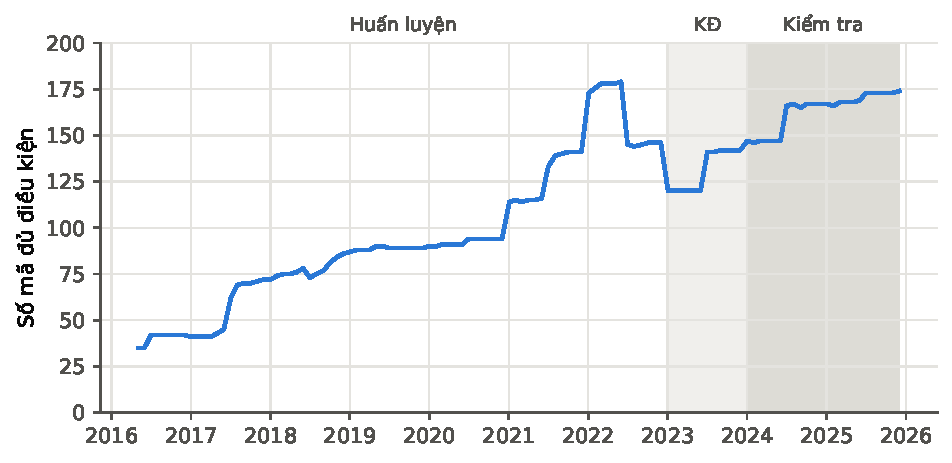
\includegraphics[width=0.88\textwidth]{eligible_universe.pdf}
\caption{Số cổ phiếu đủ điều kiện đầu tư tại mỗi ngày quyết định (tần suất tháng). Hai vùng nền xám lần lượt là giai đoạn kiểm định (2023) và kiểm tra (2024--2025).}
\label{fig:eligible}
\end{figure}

\subsection{Bộ đặc trưng}
\label{sec:features}

Mỗi cổ phiếu tại mỗi phiên được mô tả bằng $F=19$ đặc trưng thuộc ba nhóm (Bảng~\ref{tab:features}).

\begin{table}[ht]
\centering\small
\caption{Bộ 19 đặc trưng đầu vào}
\label{tab:features}
\begin{tabularx}{\textwidth}{@{}p{2.2cm}p{3.3cm}X@{}}
\toprule
Nhóm & Đặc trưng & Định nghĩa \\
\midrule
\multirow{9}{2.2cm}{Giá và kỹ thuật (9)}
 & \texttt{log\_return} & Lợi suất logarit theo ngày, công thức~\eqref{eq:logret} \\
 & \texttt{log\_volume} & Thay đổi logarit của khối lượng: $\ln(V_s/V_{s-1})$ \\
 & \texttt{volatility\_20d/60d} & Độ lệch chuẩn của lợi suất trong 20 và 60 phiên, quy năm ($\times\sqrt{252}$) \\
 & \texttt{rsi\_14} & Chỉ số sức mạnh tương đối 14 phiên \cite{wilder1978} \\
 & \texttt{momentum\_20d/60d} & $\ln(P_s/P_{s-20})$ và $\ln(P_s/P_{s-60})$ \\
 & \texttt{ma\_ratio} & Tỷ số trung bình động 20 phiên trên 50 phiên \\
 & \texttt{log\_amihud\_20d} & Logarit của độ kém thanh khoản Amihud \cite{amihud2002}: trung bình 20 phiên của $|R_s|/\text{GTGD}_s$ \\
\midrule
\multirow{5}{2.2cm}{Tài chính doanh nghiệp (5)}
 & \texttt{PE\_RATIO} & Hệ số giá trên thu nhập \\
 & \texttt{PX\_TO\_BOOK\_RATIO} & Hệ số giá trên giá trị sổ sách \\
 & \texttt{Net income growth} & Tăng trưởng lợi nhuận sau thuế lũy kế bốn quý so với cùng kỳ năm trước \\
 & \texttt{ROE} & Lợi nhuận sau thuế lũy kế bốn quý chia cho vốn chủ sở hữu \\
 & \texttt{A/E} & Đòn bẩy tài chính: tổng tài sản chia cho vốn chủ sở hữu \\
\midrule
\multirow{5}{2.2cm}{Vĩ mô (5)}
 & \texttt{inflation} & Lạm phát CPI so với cùng kỳ \\
 & \texttt{bond\_yield} & Lợi suất trái phiếu Chính phủ \\
 & \texttt{interbank\_rate} & Lãi suất liên ngân hàng qua đêm \\
 & \texttt{vnindex\_return} & Lợi suất hằng ngày của VN-Index \\
 & \texttt{usdvnd\_fx\_rate} & Tỷ giá giữa đồng Việt Nam và đô la Mỹ \\
\bottomrule
\end{tabularx}
\end{table}

\textit{Nhóm giá và kỹ thuật} mô tả xu hướng, rủi ro và thanh khoản gần đây của từng mã. Động lượng 20 và 60 phiên phản ánh hiệu ứng động lượng đã được ghi nhận rộng rãi \cite{jegadeesh1993}; hai thước đo biến động đại diện cho rủi ro riêng; độ kém thanh khoản Amihud đo mức biến động giá trên một đơn vị giá trị giao dịch và đặc biệt có ý nghĩa ở thị trường có thanh khoản phân hóa.

\textit{Nhóm tài chính doanh nghiệp} mô tả định giá, khả năng sinh lời, tăng trưởng và cơ cấu vốn. Các chỉ số tính từ báo cáo tài chính quý chỉ thay đổi khi có báo cáo mới.

\textit{Nhóm vĩ mô} mô tả môi trường chung. Các biến này có cùng giá trị cho mọi cổ phiếu trong một phiên; chúng không giúp phân biệt các mã với nhau tại một thời điểm nhưng cho mô hình biết bối cảnh thị trường.

\subsection{Tránh rò rỉ thông tin tương lai}
\label{sec:leakage}

Rò rỉ thông tin tương lai (look-ahead bias) là sai lầm phổ biến và nghiêm trọng nhất trong kiểm thử ngược. Luận văn áp dụng các nguyên tắc sau:
\begin{itemize}
  \item \textit{Gắn dữ liệu tài chính theo ngày công bố.} Các chỉ số của quý $q$ chỉ được đưa vào dữ liệu từ ngày doanh nghiệp công bố báo cáo quý $q$, không phải từ ngày kết thúc quý; sau đó giá trị được giữ nguyên (điền tiến) đến lần công bố kế tiếp.
  \item \textit{Xét vốn hóa bằng thông tin quá khứ.} Nhãn đủ điều kiện tại phiên $s$ chỉ dùng mốc xét vốn hóa gần nhất không muộn hơn $s$.
  \item \textit{Cửa sổ chỉ gồm các phiên trước ngày quyết định.} Tại ngày quyết định $t$, cả ten-xơ đặc trưng và ma trận tương quan đều được tính từ $T$ phiên có ngày \emph{nhỏ hơn hẳn} $t$.
  \item \textit{Chuẩn hóa trong cửa sổ.} Trung bình và độ lệch chuẩn dùng để chuẩn hóa được tính lại trong từng cửa sổ, không dùng thống kê của toàn bộ mẫu.
  \item \textit{Lợi suất nắm giữ bắt đầu sau ngày quyết định.} Lợi suất của kỳ $t$ được tính trên các phiên thuộc $(t,t^{+}]$, với $t^{+}$ là ngày quyết định kế tiếp (công thức~\eqref{eq:holdret}). Quy ước này tương ứng với việc quan sát dữ liệu đến hết phiên $t-1$, đặt lệnh trong phiên $t$ và được khớp tại giá đóng cửa phiên $t$.
  \item \textit{Chia dữ liệu theo thời gian, không xáo trộn.}
\end{itemize}

\subsection{Chia dữ liệu}

Trục thời gian được chia theo tỷ lệ 70\% -- 10\% -- 20\% số ngày lịch, cho ba giai đoạn liền nhau (Bảng~\ref{tab:split}). Ngày quyết định là phiên giao dịch đầu tiên của mỗi tháng (thiết lập chính) hoặc mỗi tuần (thiết lập bổ sung), tính từ khi đã có đủ 60 phiên lịch sử. Số bước quyết định dùng được ít hơn số ngày quyết định một đơn vị, vì ngày quyết định cuối cùng của mỗi tập không có kỳ nắm giữ tương ứng.

\begin{table}[ht]
\centering\small
\caption{Chia dữ liệu theo thời gian và số ngày quyết định ở hai tần suất tái cân bằng}
\label{tab:split}
\begin{tabular}{@{}lcccc@{}}
\toprule
 & & \multicolumn{2}{c}{Số ngày quyết định} & Số mã đủ điều kiện \\
\cmidrule(lr){3-4}
Tập & Giai đoạn & Tháng & Tuần & (trung bình) \\
\midrule
Huấn luyện & 04/2016 -- 12/2022 & 80 & 349 & 94 \\
Kiểm định & 01/2023 -- 12/2023 & 12 & 52 & 131 \\
Kiểm tra & 01/2024 -- 12/2025 & 24 & 104 & 164 \\
\bottomrule
\end{tabular}
\end{table}

Cần nhấn mạnh quy mô của bài toán dưới góc nhìn học tăng cường: với tái cân bằng theo tháng, toàn bộ ``kinh nghiệm'' của tác tử trong tập huấn luyện chỉ gồm 79 bước quyết định, tập kiểm định có 11 bước và tập kiểm tra có 23 bước. Đây là lượng dữ liệu rất nhỏ so với các bài toán điều khiển mà PPO thường được áp dụng, và là bối cảnh cần ghi nhớ khi diễn giải kết quả ở Chương~\ref{ch:thucnghiem}.

\section{Dựng ten-xơ đầu vào và chuẩn hóa}
\label{sec:snapshot}

Tại ngày quyết định $t$, gọi $s_1<\dots<s_T$ là $T=60$ phiên gần nhất trước $t$. Ten-xơ $X_t\in\R^{N\times T\times F}$ có phần tử $X_t[i,k,f]$ là giá trị đặc trưng $f$ của cổ phiếu $i$ tại phiên $s_k$. Các giá trị thiếu hoặc vô hạn (chẳng hạn thay đổi logarit của khối lượng khi khối lượng bằng không) được thay bằng $0$.

Hai nhóm đặc trưng được chuẩn hóa theo hai cách khác nhau, phù hợp với bản chất của chúng.

\textit{Đặc trưng theo từng mã} (14 đặc trưng thuộc nhóm giá--kỹ thuật và tài chính) được chuẩn hóa \emph{theo lát cắt ngang}: tại mỗi phiên $s_k$,
\begin{equation}
\tilde X_t[i,k,f]=\frac{X_t[i,k,f]-\mu_{k,f}}{\sigma_{k,f}},\qquad
\mu_{k,f}=\frac{1}{N_t}\sum_{j:\,m_{t,j}=1}X_t[j,k,f],
\label{eq:xsec}
\end{equation}
với $\sigma_{k,f}$ là độ lệch chuẩn tương ứng trên các mã đủ điều kiện. Sau phép biến đổi này, giá trị của một đặc trưng cho biết cổ phiếu đang ở vị trí nào \emph{so với các cổ phiếu khác trong cùng phiên} -- chẳng hạn P/E thấp hơn hay cao hơn mặt bằng chung. Cách chuẩn hóa này loại bỏ xu hướng chung của thị trường và sự trôi dạt của thang đo theo thời gian, đồng thời phù hợp với bản chất của bài toán danh mục là so sánh tương đối giữa các mã.

\textit{Đặc trưng vĩ mô} (5 đặc trưng) có cùng giá trị cho mọi mã nên không thể chuẩn hóa theo lát cắt ngang; chúng được chuẩn hóa \emph{theo thời gian} trong cửa sổ:
\begin{equation}
\tilde X_t[i,k,f]=\frac{X_t[i,k,f]-\mu_f}{\sigma_f},
\label{eq:tsnorm}
\end{equation}
với $\mu_f,\sigma_f$ tính trên 60 phiên của cửa sổ. Giá trị sau chuẩn hóa cho biết biến vĩ mô đang cao hay thấp so với chính nó trong ba tháng gần nhất.

Cuối cùng, mọi giá trị được cắt về đoạn $[-10,10]$ để hạn chế ảnh hưởng của ngoại lệ. Khi độ lệch chuẩn nhỏ hơn $10^{-8}$, nó được thay bằng $1$ để tránh chia cho số gần không.

\section{Đồ thị tương quan động}
\label{sec:graph}

\subsection{Xây dựng ma trận kề}

Đồ thị tại ngày quyết định $t$ được xây dựng chỉ từ lợi suất, tách biệt với các đặc trưng khác: mục đích của đồ thị là mô tả sự đồng biến động về giá, không phải sự tương đồng về chỉ số tài chính. Với hai cổ phiếu $i,j$, hệ số tương quan Pearson của lợi suất logarit trong cửa sổ $T_c$ phiên trước $t$ là
\begin{equation}
\rho_{ij}(t)=\corr\big(\ell_{i,s_1:s_{T_c}},\;\ell_{j,s_1:s_{T_c}}\big),
\label{eq:corr}
\end{equation}
được tính trên các phiên mà cả hai mã đều có dữ liệu; nếu số phiên chung nhỏ hơn 30 thì đặt $\rho_{ij}(t)=0$. Ma trận kề có trọng số được định nghĩa bởi
\begin{equation}
A_{ij}(t)=
\begin{cases}
|\rho_{ij}(t)|, & |\rho_{ij}(t)|\ge\tau,\; i\ne j,\\
1, & i=j,\\
0, & \text{còn lại,}
\end{cases}
\label{eq:adj}
\end{equation}
với ngưỡng $\tau=0{,}30$. Giá trị tuyệt đối được dùng vì cả tương quan dương lẫn âm mạnh đều chứa thông tin về quan hệ giữa hai mã; ngưỡng $\tau$ loại các tương quan yếu vốn chủ yếu là nhiễu ước lượng. Sau đó, các cạnh nối tới cổ phiếu không đủ điều kiện bị loại bỏ:
\begin{equation}
\bar A_{ij}(t)=A_{ij}(t)\,m_{t,i}\,m_{t,j},
\label{eq:maskadj}
\end{equation}
nên các nút này bị cô lập hoàn toàn và không tham gia truyền thông điệp.

Trong thiết lập chính, cửa sổ ước lượng trùng với cửa sổ đặc trưng, $T_c=60$ phiên. Để khảo sát quan hệ tương quan \emph{dài hạn} nêu trong tên đề tài, luận văn xét thêm biến thể $T_c=250$ phiên (khoảng một năm giao dịch). Hai lựa chọn thể hiện hai quan niệm khác nhau: cửa sổ ngắn bám sát chế độ thị trường hiện tại nhưng nhiễu hơn; cửa sổ dài cho ước lượng ổn định hơn, phản ánh quan hệ bền vững giữa các doanh nghiệp, nhưng phản ứng chậm khi cấu trúc thị trường thay đổi.

\subsection{Đặc điểm của đồ thị qua các giai đoạn thị trường}

Hình~\ref{fig:density} trình bày mật độ đồ thị -- tỷ lệ cặp cổ phiếu đủ điều kiện có cạnh nối -- theo thời gian cho hai cửa sổ. Có ba quan sát đáng chú ý.

\begin{figure}[ht]
\centering
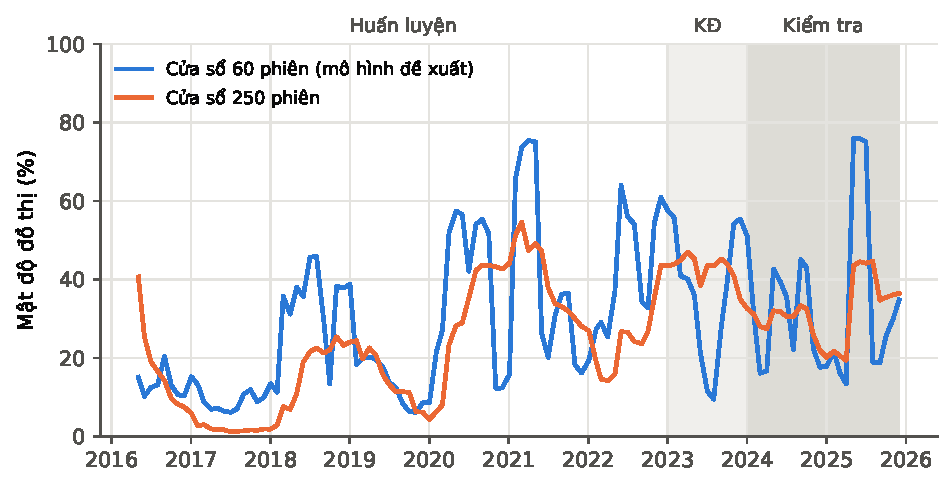
\includegraphics[width=0.9\textwidth]{graph_density.pdf}
\caption{Mật độ của đồ thị tương quan (ngưỡng $\tau=0{,}30$) theo thời gian với cửa sổ ước lượng 60 phiên và 250 phiên.}
\label{fig:density}
\end{figure}

Thứ nhất, cấu trúc đồ thị thay đổi rất mạnh. Với cửa sổ 60 phiên, mật độ trung bình là 30\% nhưng dao động từ 6\% (tháng 11/2019) đến 76\% (tháng 5/2025). Hình~\ref{fig:adjsnap} minh họa hai thái cực này: ở trạng thái thưa, đồ thị chỉ gồm một nhóm nhỏ cổ phiếu liên kết với nhau; ở trạng thái dày, gần như mọi cổ phiếu đều nối với nhau.

Thứ hai, mật độ tăng vọt trong các giai đoạn thị trường căng thẳng: quý I/2020 (COVID-19), các đợt điều chỉnh năm 2021 và 2022, và tháng 4--5/2025. Điều này nhất quán với hiện tượng tương quan tăng khi thị trường giảm mạnh đã được ghi nhận trong tài liệu \cite{longin2001}. Hệ quả đối với mô hình là trong khủng hoảng, đồ thị gần như đầy đủ và ít mang thông tin phân biệt: phép gộp trên lân cận tiến gần tới phép lấy trung bình toàn thị trường.

Thứ ba, đồ thị cửa sổ 250 phiên mượt hơn và phản ứng trễ hơn, đúng như dự đoán. Mật độ của nó duy trì ở mức cao trong khoảng một năm sau mỗi cú sốc, vì các phiên biến động mạnh còn nằm trong cửa sổ ước lượng.

\begin{figure}[ht]
\centering
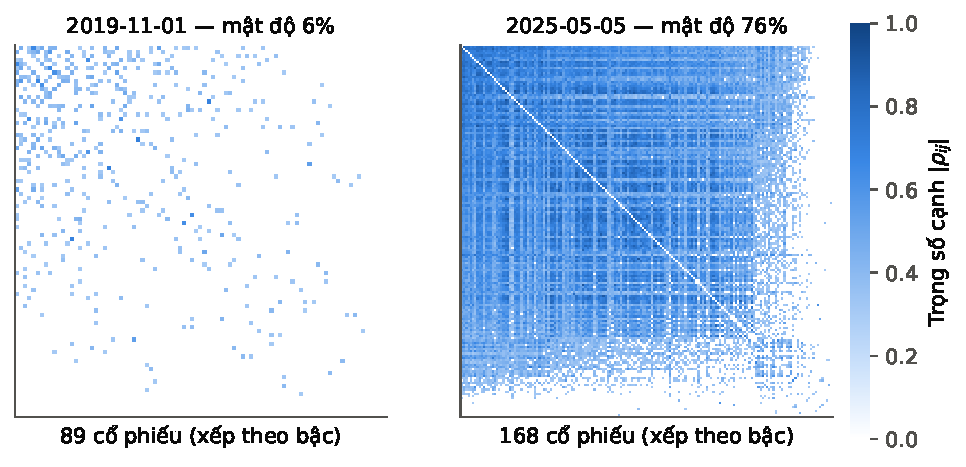
\includegraphics[width=0.95\textwidth]{adjacency_snapshots.pdf}
\caption{Ma trận kề (cửa sổ 60 phiên) tại ngày có mật độ thấp nhất và cao nhất trong giai đoạn 2019--2025. Các cổ phiếu được sắp theo bậc giảm dần; đường chéo được bỏ để dễ quan sát.}
\label{fig:adjsnap}
\end{figure}

Các quan sát này cho thấy giả định đồ thị cố định là không phù hợp với thị trường Việt Nam, và củng cố lý do dùng đồ thị được ước lượng lại theo thời gian. Đồng thời, chúng cũng chỉ ra một hạn chế của việc dùng ngưỡng cố định: số lân cận trung bình của một nút biến thiên từ dưới 3 đến hơn 120, khiến ``tầm nhìn'' của mạng đồ thị rất không đồng đều giữa các thời điểm.

\section{Bộ mã hóa thời gian}
\label{sec:encoder}

Bộ mã hóa ánh xạ chuỗi đặc trưng của mỗi cổ phiếu, $\tilde X_t[i]\in\R^{T\times F}$, thành một véc-tơ $h_i\in\R^{D}$ với $D=64$. Cùng một bộ tham số được dùng cho mọi cổ phiếu; chiều $N$ đóng vai trò chiều lô. Các bước xử lý như sau:
\begin{enumerate}[leftmargin=1.6cm]
  \item \textit{Chiếu đầu vào:} mỗi véc-tơ 19 chiều được chiếu tuyến tính lên không gian 64 chiều.
  \item \textit{Mã hóa vị trí:} cộng mã hóa vị trí dạng sin theo công thức~\eqref{eq:pe}, sau đó áp dụng dropout.
  \item \textit{Hai tầng Transformer:} mỗi tầng theo cấu trúc pre-norm~\eqref{eq:prenorm} với 4 đầu chú ý, mạng truyền thẳng 256 chiều và dropout $0{,}1$; phép chú ý dùng mặt nạ nhân quả nên biểu diễn tại phiên $s_k$ chỉ phụ thuộc vào các phiên $s_1,\dots,s_k$.
  \item \textit{Gộp theo thời gian:} lấy trung bình biểu diễn trên 60 phiên.
  \item \textit{Chiếu đầu ra:} một tầng tuyến tính và chuẩn hóa theo tầng cho $h_i$.
\end{enumerate}
Sau cùng, biểu diễn của các cổ phiếu không đủ điều kiện được đặt bằng không: $h_i\leftarrow m_{t,i}\,h_i$.

Vì toàn bộ cửa sổ đã nằm trước ngày quyết định, mặt nạ nhân quả ở đây không nhằm ngăn rò rỉ thông tin tương lai mà đóng vai trò một thiên kiến quy nạp: nó buộc mô hình xử lý chuỗi theo chiều thời gian. Bộ mã hóa Transformer có 105.536 tham số. Để phục vụ phép loại bỏ thành phần, luận văn cài đặt thêm hai bộ mã hóa hồi quy có cùng giao diện: LSTM hai tầng với 128 đơn vị ẩn (241.088 tham số) và GRU có cấu trúc tương đương (183.232 tham số), trong đó trạng thái ẩn cuối cùng của tầng trên được chiếu về 64 chiều.

\section{Mạng chú ý đồ thị}
\label{sec:gat}

Mạng đồ thị nhận ma trận biểu diễn $H=[h_1,\dots,h_N]\T$ và ma trận kề đã lọc $\bar A_t$, trả về $Z=[z_1,\dots,z_N]\T$. Luận văn tự cài đặt GAT ở dạng ma trận đặc, phù hợp với đồ thị có vài trăm nút và mật độ cao.

\textit{Tầng thứ nhất} dùng $4$ đầu chú ý, mỗi đầu có 16 chiều, tính theo các công thức~\eqref{eq:gat-e}--\eqref{eq:gat-h}; kết quả của các đầu được ghép nối thành véc-tơ 64 chiều và đưa qua hàm kích hoạt ELU:
\begin{equation}
h_i^{(1)}=\ELU\Big(\big\Vert_{k=1}^{4}\sum_{j\in\mathcal{N}(i)}\alpha_{ij}^{(k)}W^{(k)}h_j\Big).
\end{equation}
\textit{Tầng thứ hai} dùng một đầu chú ý với 64 chiều đầu ra, theo sau là chuẩn hóa theo tầng:
\begin{equation}
z_i=\LN\Big(\sum_{j\in\mathcal{N}(i)}\alpha_{ij}'\,W'h_j^{(1)}\Big).
\end{equation}
Hệ số dốc của LeakyReLU là $0{,}2$ và dropout $0{,}1$ được áp dụng lên các hệ số chú ý. Với hai tầng, biểu diễn của mỗi cổ phiếu tích hợp thông tin từ các cổ phiếu cách nó tối đa hai bước trên đồ thị. Biểu diễn của các nút không đủ điều kiện được đặt bằng không ở đầu ra.

Như đã lưu ý ở Chương~\ref{ch:lythuyet}, trong cài đặt này ma trận kề chỉ xác định tập lân cận $\mathcal{N}(i)=\{j:\bar A_{ij}\ne0\}$; độ lớn $|\rho_{ij}|$ không tham gia trực tiếp vào hệ số chú ý. Mạng GAT có 8.576 tham số.

\textit{Biến thể đối chứng.} Để đánh giá vai trò của cơ chế chú ý và của bản thân đồ thị, luận văn dùng hai biến thể: (i) GCN hai tầng theo công thức~\eqref{eq:gcn}, trong đó trọng số gộp được xác định cố định bởi $\bar A_t$ đã chuẩn hóa đối xứng (8.448 tham số) -- biến thể này \emph{có} dùng độ lớn của tương quan; và (ii) biến thể ``không đồ thị'', giữ nguyên kiến trúc GAT nhưng thay $\bar A_t$ bằng ma trận chỉ có khuyên, nên mỗi cổ phiếu không nhận thông tin từ cổ phiếu khác.

\section{Tác tử và không gian hành động}
\label{sec:agent}

\subsection{Trạng thái, hành động và chính sách}

\textit{Trạng thái} tại bước $t$ là ma trận biểu diễn $Z_t\in\R^{N\times D}$ cùng mặt nạ $m_t$. \textit{Hành động} là véc-tơ tỷ trọng $w_t$ trên các mã đủ điều kiện.

\textit{Actor} là một mạng hai tầng (64 đơn vị ẩn, kích hoạt ReLU) áp dụng riêng rẽ cho từng cổ phiếu với tham số dùng chung, cho một điểm số vô hướng $u_i$; điểm số được biến đổi thành tham số tập trung dương
\begin{equation}
\alpha_i=\softplus(u_i)+10^{-3}.
\label{eq:alpha}
\end{equation}
Chính sách là phân phối Dirichlet trên các mã đủ điều kiện (Mục~\ref{sec:dirichlet}):
\begin{equation}
w_t\big|_{\{i:\,m_{t,i}=1\}}\sim\Dir\big(\alpha_i:\,m_{t,i}=1\big),\qquad w_{t,i}=0\ \text{nếu}\ m_{t,i}=0 .
\label{eq:policy}
\end{equation}
Khi huấn luyện, $w_t$ được lấy mẫu từ phân phối này để khám phá; khi đánh giá, hành động tất định là kỳ vọng $w_{t,i}=\alpha_i/\sum_j\alpha_j$ theo~\eqref{eq:dir-mean}. Vì actor chấm điểm từng mã bằng cùng một mạng, chính sách không phụ thuộc vào số lượng hay thứ tự của các cổ phiếu, phù hợp với tập cổ phiếu thay đổi theo thời gian.

\textit{Critic} ước lượng giá trị của trạng thái từ biểu diễn trung bình của các mã đủ điều kiện:
\begin{equation}
V_\phi(s_t)=g_\phi\Big(\frac{1}{N_t}\sum_{i:\,m_{t,i}=1}z_i\Big),
\end{equation}
với $g_\phi$ là mạng hai tầng có 64 đơn vị ẩn. Actor và critic có tổng cộng 8.450 tham số; toàn bộ mô hình có khoảng 122,6 nghìn tham số.

\subsection{Chiếu về tập danh mục khả thi}
\label{sec:projection}

Một mẫu Dirichlet phân bổ tỷ trọng dương cho mọi mã đủ điều kiện, trong khi danh mục thực tế bị giới hạn về số mã và mức tập trung. Do đó $w_t$ được chiếu về tập khả thi bằng một phép biến đổi tất định $\Pi_{K,w_{\max}}$:
\begin{enumerate}[leftmargin=1.6cm]
  \item giữ lại $K=20$ mã có tỷ trọng lớn nhất, đặt các mã còn lại bằng không, rồi chuẩn hóa để tổng bằng 1;
  \item nếu có mã vượt trần $w_{\max}=10\%$, cắt mã đó về $w_{\max}$ và phân phối phần dư cho các mã chưa chạm trần theo tỷ lệ tỷ trọng hiện có; lặp lại đến khi không còn mã nào vượt trần.
\end{enumerate}
Với $K=20$ và $w_{\max}=10\%$, mỗi mã được nắm giữ có tỷ trọng trung bình 5\% và không quá 10\%.

Về mặt hình thức, phép chiếu được coi là \emph{một phần của môi trường}: hành động của tác tử vẫn là mẫu Dirichlet $w_t$ (dùng để tính xác suất trong hàm mục tiêu PPO), còn môi trường thực thi danh mục $\tilde w_t=\Pi_{K,w_{\max}}(w_t)$ và trả về phần thưởng tương ứng. Cách xử lý này hợp lệ đối với thuật toán gradient chính sách, nhưng nó tạo ra một ánh xạ nhiều--một từ hành động sang danh mục thực thi; ảnh hưởng của điều này đến việc học được phân tích ở Mục~\ref{sec:policy-behaviour}.

\subsection{Phần thưởng}

Lợi suất ròng của bước $t$ được tính theo~\eqref{eq:netret} với danh mục thực thi:
\begin{equation}
r_t=\tilde w_t\T R_t-c\,\lVert\tilde w_t-\tilde w_{t-1}\rVert_1,\qquad c=10\ \text{điểm cơ bản},
\end{equation}
trong đó $R_t$ là véc-tơ lợi suất nắm giữ trong kỳ; cổ phiếu không có dữ liệu giá trong kỳ được gán lợi suất bằng không. Phần thưởng là tỷ số Sharpe vi phân~\eqref{eq:dsr} của chuỗi $r_t$ với $\eta=0{,}01$. Ở bước đầu tiên của mỗi quỹ đạo, các mô-men được khởi tạo $A_1=r_1$, $B_1=r_1^2$ và phần thưởng bằng không; khi phương sai trượt nhỏ hơn ngưỡng số học, phần thưởng cũng được đặt bằng không. Cuối cùng, phần thưởng được cắt về đoạn $[-5,5]$:
\begin{equation}
\text{phần thưởng}_t=\clip(D_t,-5,5).
\label{eq:reward}
\end{equation}

\section{Quy trình huấn luyện đầu--cuối}
\label{sec:training}

Thuật toán~\ref{alg:train} tóm tắt quy trình huấn luyện. Mỗi vòng lặp gồm hai pha.

\textit{Pha thu thập (rollout).} Tác tử chạy tuần tự qua toàn bộ các ngày quyết định của tập huấn luyện theo thứ tự thời gian, tạo thành \emph{một} quỹ đạo. Tại mỗi bước, mô hình tính $Z_t$, lấy mẫu hành động, môi trường trả về lợi suất ròng và phần thưởng. Pha này không tính gradient; hành động, logarit xác suất và giá trị ước lượng được lưu lại.

\textit{Pha cập nhật.} Lợi thế được tính bằng GAE~\eqref{eq:gae} với $\gamma=0{,}99$, $\lambda=0{,}95$ rồi chuẩn hóa về trung bình không và phương sai đơn vị. Trong mỗi epoch, phép tính xuôi qua bộ mã hóa và mạng đồ thị được \emph{thực hiện lại} cho từng bước để gradient của hàm mất mát~\eqref{eq:ppo-loss} truyền ngược qua cả ba khối; gradient được cộng dồn trên toàn bộ quỹ đạo, cắt chuẩn về 1 rồi cập nhật một lần bằng Adam \cite{kingma2015}. Như vậy mỗi vòng lặp gồm $E_{\mathrm{ppo}}=4$ bước gradient trên toàn lô.

\textit{Chọn mô hình.} Sau mỗi vòng lặp, chính sách tất định được chạy trên tập kiểm định và tỷ số Sharpe quy năm được ghi lại; bộ tham số có tỷ số Sharpe kiểm định cao nhất được giữ làm mô hình cuối cùng.

\begin{algorithm}[ht]
\caption{Huấn luyện đầu--cuối mô hình Transformer--GAT--PPO}
\label{alg:train}
\small
\begin{algorithmic}[1]
\Require Dữ liệu huấn luyện và kiểm định; phí $c$; ngưỡng cắt $\epsilon$; số vòng lặp $N_{\mathrm{iter}}$; số epoch $E_{\mathrm{ppo}}$
\Ensure Tham số $\theta^{*}$ của bộ mã hóa $f_{\mathrm{enc}}$, mạng đồ thị $f_{\mathrm{gat}}$ và tác tử $(\pi,V)$
\State Dựng trước $(X_t,m_t,\bar A_t,R_t)$ cho mọi ngày quyết định $t$
\For{vòng lặp $=1,\dots,N_{\mathrm{iter}}$}
  \State Khởi tạo lại bộ ước lượng DSR; $\tilde w_{0}\gets 0$
  \For{mỗi ngày quyết định $t$ của tập huấn luyện} \Comment{pha thu thập, không gradient}
    \State $Z_t\gets f_{\mathrm{gat}}\big(m_t\odot f_{\mathrm{enc}}(X_t),\bar A_t\big)$
    \State Lấy mẫu $w_t\sim\Dir(\alpha(Z_t))$; lưu $\log\pi(w_t\mid Z_t)$ và $V(Z_t)$
    \State $\tilde w_t\gets\Pi_{K,w_{\max}}(w_t)$;\quad $r_t\gets\tilde w_t\T R_t-c\lVert\tilde w_t-\tilde w_{t-1}\rVert_1$
    \State Phần thưởng $\gets\clip(D_t,-5,5)$ với $D_t$ theo~\eqref{eq:dsr}
  \EndFor
  \State Tính lợi thế $\hat A_t$ bằng GAE và mục tiêu $\hat G_t$; chuẩn hóa $\hat A_t$
  \For{epoch $=1,\dots,E_{\mathrm{ppo}}$} \Comment{pha cập nhật}
    \State Tính lại $Z_t$ có gradient cho mọi $t$; cộng dồn gradient của hàm mất mát~\eqref{eq:ppo-loss}
    \State Cắt chuẩn gradient về 1; cập nhật $\theta$ bằng Adam
  \EndFor
  \State Tính tỷ số Sharpe của chính sách tất định trên tập kiểm định; lưu $\theta$ nếu tốt nhất
\EndFor
\State \Return bộ tham số có tỷ số Sharpe kiểm định cao nhất
\end{algorithmic}
\end{algorithm}

Bảng~\ref{tab:hyper} liệt kê các siêu tham số. Chúng được giữ cố định cho mọi thực nghiệm; luận văn không tinh chỉnh siêu tham số trên tập kiểm tra.

\begin{table}[ht]
\centering\small
\caption{Cấu hình mô hình và siêu tham số huấn luyện}
\label{tab:hyper}
\begin{tabular}{@{}llp{6.4cm}@{}}
\toprule
Thành phần & Tham số & Giá trị \\
\midrule
Dữ liệu & Cửa sổ đặc trưng $T$; số đặc trưng $F$ & 60 phiên; 19 \\
 & Ràng buộc danh mục & $K=20$ mã, $w_{\max}=10\%$ \\
 & Phí giao dịch $c$ & 10 điểm cơ bản trên giá trị luân chuyển \\
Đồ thị & Thước đo; cửa sổ; ngưỡng & $|\rho|$ Pearson; 60 phiên (biến thể: 250); $\tau=0{,}30$ \\
 & Số quan sát chung tối thiểu & 30 phiên \\
Bộ mã hóa & Kiến trúc & Transformer pre-norm, 2 tầng, 4 đầu, $d=64$, FFN 256 \\
 & Gộp; dropout & trung bình theo thời gian; $0{,}1$ \\
GAT & Tầng 1 / tầng 2 & 4 đầu $\times$ 16 chiều (ghép), ELU / 1 đầu $\times$ 64 chiều \\
Tác tử & Actor / critic & MLP 64--64--1 (theo từng mã) / MLP 64--64--1 (sau gộp trung bình) \\
 & Chính sách & Dirichlet, $\alpha_i=\softplus(u_i)+10^{-3}$ \\
PPO & $\epsilon$; epoch mỗi vòng; $\gamma$; $\lambda$ & $0{,}2$; 4; $0{,}99$; $0{,}95$ \\
 & $c_v$; $c_e$; cắt gradient & $0{,}5$; $0{,}01$; chuẩn $\le 1$ \\
 & Bộ tối ưu; tốc độ học & Adam; $3\times10^{-4}$ \\
Phần thưởng & DSR: $\eta$; biên độ cắt & $0{,}01$; $\pm5$ \\
Chọn mô hình & Tiêu chí & Tỷ số Sharpe cao nhất trên tập kiểm định \\
\bottomrule
\end{tabular}
\end{table}

\section{Tổng kết chương}

Chương này đã mô tả bộ dữ liệu 222 mã cổ phiếu Việt Nam giai đoạn 2016--2025 với 19 đặc trưng thuộc ba nhóm, cùng các nguyên tắc xử lý nhằm tránh rò rỉ thông tin tương lai. Tập cổ phiếu đủ điều kiện thay đổi theo thời gian, từ 35 đến 179 mã. Đồ thị tương quan được ước lượng lại tại mỗi ngày quyết định; khảo sát cho thấy mật độ của nó biến thiên từ 6\% đến 76\% và tăng vọt trong các giai đoạn thị trường căng thẳng. Mô hình đề xuất ghép ba khối -- bộ mã hóa Transformer, mạng GAT hai tầng và tác tử PPO với chính sách Dirichlet -- thành một hệ thống khoảng 122,6 nghìn tham số, huấn luyện đầu--cuối với phần thưởng là tỷ số Sharpe vi phân sau phí giao dịch. Chương tiếp theo trình bày thực nghiệm và kết quả.

\chapter{THỰC NGHIỆM VÀ ĐÁNH GIÁ KẾT QUẢ}
\label{ch:thucnghiem}

Chương này trình bày thiết lập thực nghiệm và kết quả. Mục~\ref{sec:setup} mô tả giao thức đánh giá, các chiến lược đối chứng và các biến thể của mô hình. Mục~\ref{sec:overall} trình bày kết quả tổng thể trên tập kiểm tra. Các mục tiếp theo phân tích độ biến động theo hạt giống, so sánh với danh mục ngẫu nhiên và mạng chưa huấn luyện, phép loại bỏ thành phần, quá trình huấn luyện, hành vi của chính sách, thiết lập tái cân bằng theo tuần và độ vững của kết quả trước lỗi dữ liệu giá.

\section{Thiết lập thực nghiệm}
\label{sec:setup}

\subsection{Giao thức đánh giá}

Mọi chiến lược được đánh giá bằng cùng một quy trình kiểm thử ngược trên tập kiểm tra từ tháng 01/2024 đến tháng 12/2025. Tại mỗi ngày quyết định $t$, chiến lược chọn véc-tơ tỷ trọng chỉ dựa trên dữ liệu trước $t$; danh mục được nắm giữ đến ngày quyết định kế tiếp; lợi suất ròng được tính theo công thức~\eqref{eq:netret} với phí 10 điểm cơ bản trên giá trị luân chuyển. Từ chuỗi lợi suất ròng, luận văn tính các chỉ số ở Mục~\ref{sec:metrics}: tỷ số Sharpe quy năm, lợi suất tích lũy, độ biến động quy năm, mức sụt giảm tối đa (MDD), tỷ số Calmar và mức luân chuyển trung bình mỗi kỳ.

Thiết lập chính dùng tái cân bằng theo tháng, cho 23 kỳ nắm giữ trên tập kiểm tra. Đây cũng là thiết lập của bài báo đã công bố \cite{tran2026dynamic}. Thiết lập tái cân bằng theo tuần (103 kỳ) được trình bày riêng ở Mục~\ref{sec:weekly}.

Với mô hình học tăng cường, mỗi cấu hình được huấn luyện độc lập với nhiều hạt giống ngẫu nhiên; hạt giống quyết định cả giá trị khởi tạo của mạng lẫn các hành động được lấy mẫu trong pha thu thập. Kết quả được báo cáo dưới dạng trung bình $\pm$ độ lệch chuẩn mẫu trên các hạt giống. Mỗi lần huấn luyện gồm $N_{\mathrm{iter}}=8$ vòng lặp PPO, tức 32 bước cập nhật gradient; mô hình được chọn là mô hình có tỷ số Sharpe kiểm định cao nhất trong 8 vòng. Các siêu tham số khác theo Bảng~\ref{tab:hyper}.

\subsection{Các chiến lược đối chứng}
\label{sec:baselines}

Luận văn so sánh mô hình đề xuất với ba nhóm đối chứng.

\textit{Nhóm 1 -- chiến lược thụ động và truyền thống:}
\begin{itemize}
  \item \textbf{Phân bổ đều (1/N):} chia đều vốn cho mọi cổ phiếu đủ điều kiện tại mỗi ngày quyết định. Đây là mốc so sánh quan trọng nhất vì nó dùng đúng tập cổ phiếu và đúng dữ liệu giá của mô hình, chỉ khác ở chỗ không lựa chọn.
  \item \textbf{VN-Index:} mua và nắm giữ chỉ số, không chịu phí. Cần lưu ý ba điểm khi so sánh với VN-Index: chỉ số được tính theo tỷ trọng vốn hóa nên không chịu giới hạn 10\% mỗi mã; chỉ số chỉ gồm cổ phiếu HOSE trong khi tập cổ phiếu của luận văn rộng hơn; và chỉ số đã được điều chỉnh theo các sự kiện doanh nghiệp trong khi dữ liệu giá từng mã thì chưa (Mục~\ref{sec:robust-clean}).
  \item \textbf{Phương sai nhỏ nhất} và \textbf{trung bình--phương sai (danh mục tiếp tuyến)} của Markowitz: lợi suất kỳ vọng là trung bình mẫu và ma trận hiệp phương sai là ước lượng co rút Ledoit--Wolf~\eqref{eq:lw}, cùng tính trên 250 phiên trước ngày quyết định; ràng buộc chỉ mua, trần 10\% mỗi mã; bài toán tối ưu được giải bằng quy hoạch toàn phương tuần tự.
  \item \textbf{Động lượng top-20:} chia đều vốn cho 20 mã đủ điều kiện có động lượng 60 phiên cao nhất.
\end{itemize}

\textit{Nhóm 2 -- đối chứng ``không có kỹ năng'':} Một mô hình chọn 20 mã trong khoảng 160 mã luôn cho một kết quả nào đó; câu hỏi là kết quả ấy có khác với việc chọn mò hay không. Luận văn dùng hai đối chứng:
\begin{itemize}
  \item \textbf{Danh mục 20 mã ngẫu nhiên:} 1.000 danh mục, mỗi danh mục chia đều vốn cho 20 mã đủ điều kiện được chọn ngẫu nhiên. Ở biến thể ``giữ nguyên'', 20 mã được chọn một lần và chỉ thay khi một mã không còn đủ điều kiện, nên chi phí giao dịch thấp; ở biến thể ``đổi mỗi kỳ'', 20 mã được chọn lại hoàn toàn tại mỗi ngày quyết định, nên chi phí giao dịch cao. Hai biến thể kẹp hai đầu mức luân chuyển có thể có của một chiến lược chọn 20 mã.
  \item \textbf{Mạng chưa huấn luyện:} 30 bộ tham số Transformer + GAT + tác tử được khởi tạo ngẫu nhiên và dùng ngay để ra quyết định trên tập kiểm tra, không qua bước huấn luyện nào. Đối chứng này trả lời trực tiếp câu hỏi: quá trình huấn luyện PPO có cải thiện chính sách so với điểm xuất phát hay không.
\end{itemize}

\textit{Nhóm 3 -- các biến thể của mô hình (phép loại bỏ thành phần):}
\begin{itemize}
  \item \textbf{LSTM + GAT:} thay bộ mã hóa Transformer bằng LSTM, nhằm đánh giá vai trò của cơ chế tự chú ý theo thời gian.
  \item \textbf{Transformer + GCN:} thay GAT bằng GCN, nhằm đánh giá vai trò của trọng số chú ý học được so với trọng số gộp cố định.
  \item \textbf{Transformer, không đồ thị:} chỉ giữ khuyên trong ma trận kề, nhằm đánh giá vai trò của thông tin liên cổ phiếu.
  \item \textbf{Transformer + GAT với đồ thị 250 phiên:} thay cửa sổ ước lượng tương quan 60 phiên bằng 250 phiên, nhằm so sánh quan hệ tương quan ngắn hạn và dài hạn.
  \item \textbf{LSTM thuần} và \textbf{GRU thuần:} bộ mã hóa hồi quy không dùng đồ thị, với cùng tác tử PPO -- tương ứng với các mô hình học sâu chuỗi thời gian đơn lẻ nêu trong đề cương.
\end{itemize}
Mô hình đề xuất và ba biến thể đầu được huấn luyện với 5 hạt giống; ba biến thể còn lại với 3 hạt giống. Mọi biến thể dùng chung siêu tham số, tập dữ liệu và ràng buộc danh mục.


\chapter{Stub}\label{ch:x06_thaoluan} x

\chapter*{KẾT LUẬN VÀ HƯỚNG NGHIÊN CỨU TIẾP THEO}
\addcontentsline{toc}{chapter}{Kết luận và hướng nghiên cứu tiếp theo}
\markboth{KẾT LUẬN}{KẾT LUẬN}

\section*{1. Kết luận của luận văn}

Luận văn đã nghiên cứu tính khả thi của một mô hình học sâu lai, kết hợp mạng nơ-ron đồ thị với học tăng cường, trong bài toán phân bổ danh mục cho nhóm cổ phiếu có quan hệ tương quan dài hạn tại thị trường chứng khoán Việt Nam. Mục tiêu của luận văn không phải là tạo ra một hệ thống giao dịch vượt trội thị trường, mà là kiểm chứng xem phương pháp có thể được xây dựng và vận hành đúng đắn trên dữ liệu thực hay không, đánh giá khách quan hành vi của nó và xác định các điều kiện cần cho việc phát triển tiếp theo.

Về dữ liệu, luận văn đã xây dựng một bộ dữ liệu gồm 222 mã cổ phiếu vốn hóa vừa và lớn trong giai đoạn 2016--2025 với 19 đặc trưng thuộc ba nhóm: giá và kỹ thuật, tài chính doanh nghiệp, vĩ mô. Chuỗi giá được điều chỉnh theo các sự kiện doanh nghiệp bằng phép đối chiếu chéo với hệ số P/B; chỉ số tài chính được gắn theo ngày công bố; tập cổ phiếu đủ điều kiện được xác định lại định kỳ bằng thông tin quá khứ.

Về quan hệ tương quan dài hạn, luận văn đã chỉ ra bằng dữ liệu rằng quan hệ này tồn tại, có cấu trúc và bền vững trên thị trường Việt Nam. Các nhóm cổ phiếu tìm được hoàn toàn từ tương quan lợi suất giai đoạn 2016--2022 trùng với các nhóm ngành thép, chứng khoán, dầu khí, ngân hàng và bất động sản. Trong các cặp cổ phiếu có tương quan từ 0,30 trở lên ở giai đoạn này, 76\% tiếp tục có tương quan từ 0,30 trở lên ở giai đoạn 2024--2025. Đồ thị tương quan ước lượng trên 250 phiên giữ được trung bình 81\% tập cạnh qua mỗi tháng, so với 52\% của đồ thị 60 phiên.

Về mô hình, luận văn đã thiết kế và cài đặt một kiến trúc huấn luyện đầu--cuối gồm bộ mã hóa Transformer có mặt nạ nhân quả, mạng chú ý đồ thị hai tầng trên đồ thị tương quan dài hạn và tác tử PPO với chính sách Dirichlet, phần thưởng là tỷ số Sharpe vi phân tính trên lợi suất ròng sau phí giao dịch. Mô hình xử lý được tập cổ phiếu thay đổi theo thời gian và luôn tạo ra danh mục thỏa mãn ràng buộc.

Về kết quả thực nghiệm trên giai đoạn kiểm tra 2024--2025, có thể rút ra bốn kết luận:
\begin{itemize}
  \item \textit{Phương pháp khả thi.} Mô hình với đồ thị tương quan dài hạn đạt tỷ số Sharpe $1{,}32\pm0{,}24$, lợi suất tích lũy 36,8\% và mức sụt giảm tối đa $-5{,}9\%$ trên 5 hạt giống ngẫu nhiên, tốt hơn danh mục phân bổ đều (0,90; 28,0\%; $-8{,}9\%$) ở mọi hạt giống và nằm trong khoảng phân vị 84--99,5\% của phân phối danh mục ngẫu nhiên. Mỗi lần huấn luyện mất dưới 15 phút trên CPU.
  \item \textit{Quan hệ tương quan dài hạn là thành phần có giá trị nhất.} So với đồ thị ngắn hạn 60 phiên, đồ thị dài hạn nâng tỷ số Sharpe trung bình từ 0,70 lên 1,32 và giảm một nửa mức luân chuyển. So với mô hình không dùng đồ thị, nó giảm khoảng một phần ba độ biến động và một nửa mức sụt giảm tối đa, ở cả bộ mã hóa Transformer lẫn LSTM. Lợi ích này đến từ cơ chế đa dạng hóa: đồ thị dài hạn giúp mô hình nhận ra và ưu tiên các cổ phiếu ít liên kết với phần còn lại của thị trường.
  \item \textit{Mô hình chưa vượt các mốc so sánh mạnh nhất.} Tỷ số Sharpe trung bình còn thấp hơn VN-Index (1,45) và danh mục trung bình--phương sai với hiệp phương sai co rút (1,56). Với 23 quan sát hằng tháng, sai số chuẩn của tỷ số Sharpe vào khoảng 0,75, nên các chênh lệch này -- cũng như chênh lệch so với phân bổ đều -- chưa có ý nghĩa thống kê.
  \item \textit{Đóng góp của học tăng cường còn hạn chế.} Mạng chưa huấn luyện trên cùng kiến trúc và cùng đồ thị dài hạn đạt tỷ số Sharpe $1{,}27\pm0{,}36$, không khác biệt về trung bình so với mô hình đã huấn luyện. Với 79 bước quyết định theo tháng, tác tử chưa có đủ kinh nghiệm để học; chính sách hiện mới đóng vai trò chọn cổ phiếu, chưa phân bổ tỷ trọng.
\end{itemize}

Như vậy, câu trả lời cho câu hỏi nghiên cứu là: việc kết hợp mạng nơ-ron đồ thị trên quan hệ tương quan dài hạn với học tăng cường để phân bổ danh mục cổ phiếu Việt Nam là khả thi và có cơ sở; giá trị đã được xác nhận nằm ở cấu trúc đồ thị dài hạn, còn giá trị của thành phần học tăng cường cần thêm dữ liệu và cải tiến về thiết kế bài toán học mới có thể khẳng định.

\section*{2. Hạn chế}

Các kết luận trên cần được hiểu trong các giới hạn sau. Giai đoạn kiểm tra chỉ dài hai năm và không có thị trường giảm kéo dài. Danh mục của mô hình nghiêng về các cổ phiếu kém thanh khoản, trong khi mô hình chi phí chỉ gồm phí tuyến tính 10 điểm cơ bản và chưa xét tác động giá hay giới hạn khối lượng; hiệu quả thực tế khi triển khai có thể thấp hơn. Phép điều chỉnh giá chỉ xử lý được các sự kiện doanh nghiệp lớn và chưa tính cổ tức tiền mặt. Tập cổ phiếu không gồm các mã đã hủy niêm yết. Quy mô huấn luyện nhỏ và chưa có tinh chỉnh siêu tham số. Dữ liệu tin tức chưa được tích hợp, và quan hệ dài hạn mới được đo bằng tương quan Pearson.

\section*{3. Hướng nghiên cứu tiếp theo}

Từ các kết quả và hạn chế trên, luận văn đề xuất các hướng nghiên cứu sau.

\textit{Kiểm chứng trên tập cổ phiếu có thanh khoản tốt.} Bổ sung bộ lọc thanh khoản vào điều kiện đủ điều kiện và mô hình chi phí phụ thuộc thanh khoản, để xác nhận lợi ích của đồ thị dài hạn trong điều kiện có thể giao dịch thực tế.

\textit{Phát triển biểu diễn quan hệ dài hạn.} Xây dựng đồ thị từ tương quan của phần dư sau khi loại thành phần thị trường; kéo dài cửa sổ ước lượng; kết hợp đồ thị dài hạn với đồ thị ngắn hạn; và khảo sát các thước đo khác như đồng liên kết, DTW hay quan hệ dẫn--trễ.

\textit{Tăng hiệu quả của học tăng cường.} Tạo thêm quỹ đạo huấn luyện bằng các ngày quyết định lệch pha và lấy mẫu tập con cổ phiếu; dùng phần thưởng tương đối so với danh mục phân bổ đều; thiết kế lại không gian hành động để tác tử học được cả lựa chọn lẫn tỷ trọng; tiền huấn luyện bộ mã hóa và mạng đồ thị bằng một nhiệm vụ có giám sát.

\textit{Mở rộng dữ liệu và đánh giá.} Tích hợp đặc trưng từ tin tức tài chính như đề cương đã dự kiến; dùng chuỗi giá điều chỉnh đầy đủ kèm cổ tức; đánh giá bằng kiểm định tiến cuốn chiếu trên nhiều giai đoạn, bao gồm các năm thị trường giảm; và tăng số hạt giống để có các khoảng tin cậy hẹp hơn.


\printbibliography

\appendix
\titleformat{\chapter}[display]{\normalfont\bfseries\centering\large}{PHỤ LỤC \thechapter}{4pt}{\Large\MakeUppercase}
\renewcommand{\cftchappresnum}{PHỤ LỤC }
\chapter{MÃ NGUỒN VÀ HƯỚNG DẪN TÁI LẬP KẾT QUẢ}
\label{app:code}

\section{Cấu trúc mã nguồn}

Toàn bộ mã nguồn của luận văn được viết bằng Python với thư viện PyTorch. Bảng~\ref{tab:files} liệt kê các tệp chính và vai trò của chúng. Sáu tệp đầu là mã nguồn của mô hình; các tệp trong thư mục \texttt{experiments/} là các kịch bản thực nghiệm bổ sung cho luận văn, chỉ \emph{gọi} mã nguồn mô hình mà không sửa đổi nó.

\begin{table}[ht]
\centering\small
\caption{Các tệp mã nguồn chính}
\label{tab:files}
\begin{tabularx}{\textwidth}{@{}p{5.3cm}X@{}}
\toprule
Tệp & Nội dung \\
\midrule
\texttt{Full\_code\_model.ipynb} & Thu thập dữ liệu, tính chỉ báo kỹ thuật và chỉ số tài chính, gắn nhãn đủ điều kiện, ghép thành bảng dữ liệu cuối; gọi huấn luyện và đánh giá. \\
\texttt{temporal\_encoder.py} & Chia dữ liệu theo thời gian; dựng ten-xơ đầu vào và chuẩn hóa; bộ mã hóa Transformer và LSTM. \\
\texttt{adjacency.py} & Xây dựng ma trận kề từ tương quan lợi suất; lọc theo mặt nạ; chuẩn hóa cho GCN. \\
\texttt{gnn.py} & Cài đặt GAT và GCN ở dạng ma trận đặc. \\
\texttt{rl\_agent.py} & Tác tử actor--critic với chính sách Dirichlet; phép chiếu về tập danh mục khả thi. \\
\texttt{train.py} & Tỷ số Sharpe vi phân, GAE, vòng lặp PPO đầu--cuối, chọn mô hình theo tập kiểm định, lưu và nạp mô hình. \\
\texttt{evaluate.py} & Kiểm thử ngược; so sánh với phân bổ đều và VN-Index; kiểm tra tỷ trọng. \\
\midrule
\texttt{experiments/build\_dataset.py} & Dựng lại bảng dữ liệu cuối từ các tệp đã lưu, không cần gọi API. \\
\texttt{experiments/build\_cache.py} & Dựng trước ten-xơ đầu vào và ma trận kề cho mọi ngày quyết định. \\
\texttt{experiments/run\_experiments.py} & Huấn luyện mô hình đề xuất và các biến thể trên nhiều hạt giống. \\
\texttt{experiments/baselines.py} & Các chiến lược đối chứng: phân bổ đều, VN-Index, phương sai nhỏ nhất, trung bình--phương sai, động lượng, danh mục ngẫu nhiên. \\
\texttt{experiments/untrained.py} & Đối chứng mạng khởi tạo ngẫu nhiên, không huấn luyện. \\
\texttt{experiments/robustness\_clean.py} & Kiểm tra độ vững với lợi suất đã loại các sự kiện doanh nghiệp. \\
\texttt{experiments/analysis\_*.py}, \texttt{make\_tables.py} & Tổng hợp kết quả, vẽ hình và sinh bảng của luận văn. \\
\bottomrule
\end{tabularx}
\end{table}

\section{Các bước tái lập}

Các kết quả của Chương~\ref{ch:thucnghiem} được tái lập bằng chuỗi lệnh sau (chạy trong thư mục \texttt{experiments/}):

{\small\begin{verbatim}
python build_dataset.py      # bang du lieu cuoi (554.556 dong, 222 ma)
python build_cache.py        # ten-xo dau vao va ma tran ke cho moi ngay quyet dinh
python run_experiments.py    # huan luyen: 7 cau hinh, nhieu hat giong (CPU)
python baselines.py          # cac chien luoc doi chung
python baselines.py clean    # doi chung voi loi suat da hieu chinh
python untrained.py          # mang chua huan luyen
python analysis_data.py      # hinh va thong ke Chuong 3
python analysis_results.py   # hinh va thong ke Chuong 4
python robustness_clean.py   # kiem tra do vung
python make_tables.py        # sinh cac bang LaTeX
\end{verbatim}}

Hai phép kiểm chứng tính đúng đắn của quy trình tái lập đã được thực hiện. Thứ nhất, bảng dữ liệu dựng lại có đúng 554.556 dòng như kết quả lưu trong sổ tay gốc. Thứ hai, khi nạp mô hình đã huấn luyện ở tần suất tuần (\texttt{model\_weekly.pt}) và đánh giá trên tập kiểm tra, các chỉ số thu được trùng khớp với kết quả lưu trong sổ tay gốc đến chữ số thập phân cuối cùng được in ra (lợi suất tích lũy 18,4\%, tỷ số Sharpe 0,53, mức sụt giảm tối đa $-14{,}6\%$).

Các thực nghiệm trong luận văn được chạy trên CPU; mỗi lần huấn luyện mô hình Transformer + GAT ở tần suất tháng với 8 vòng lặp PPO mất khoảng 25--30 phút trên một nhân xử lý. Với hạt giống 1 và 2, kết quả thu được trên CPU trùng với kết quả đã công bố trong bài báo \cite{tran2026dynamic}.

\chapter{THỐNG KÊ MÔ TẢ VÀ KẾT QUẢ CHI TIẾT}
\label{app:detail}

\section{Thống kê mô tả các đặc trưng}

Bảng~\ref{tab:featdesc} trình bày thống kê mô tả của 19 đặc trưng \emph{trước khi chuẩn hóa}, tính trên các quan sát (ngày--cổ phiếu) đủ điều kiện trong toàn bộ giai đoạn 2016--2025. Cột cuối cho biết tỷ lệ giá trị thiếu.

\begin{table}[ht]
\centering\footnotesize
\caption{Thống kê mô tả các đặc trưng trên các quan sát đủ điều kiện (trước chuẩn hóa)}
\label{tab:featdesc}
\begin{tabular}{@{}lrrrrrr@{}}
\toprule
Đặc trưng & Trung bình & Độ lệch chuẩn & Nhỏ nhất & Trung vị & Lớn nhất & Thiếu (\%) \\
\midrule
\texttt{log\_return} & $-$0{,}000 & 0{,}026 & $-$0{,}509 & 0{,}000 & 0{,}509 & 0{,}1 \\
\texttt{log\_volume} & $-$0{,}384 & 3{,}73 & $-$44{,}29 & $-$0{,}020 & 10{,}03 & 0{,}1 \\
\texttt{volatility\_20d} & 0{,}357 & 0{,}203 & 0{,}000 & 0{,}314 & 2{,}79 & 0{,}1 \\
\texttt{volatility\_60d} & 0{,}372 & 0{,}174 & 0{,}000 & 0{,}343 & 1{,}69 & 0{,}1 \\
\texttt{rsi\_14} & 50{,}13 & 12{,}96 & 0{,}000 & 49{,}63 & 100{,}0 & 0{,}1 \\
\texttt{momentum\_20d} & 0{,}001 & 0{,}118 & $-$1{,}40 & 0{,}000 & 1{,}30 & 0{,}1 \\
\texttt{momentum\_60d} & 0{,}008 & 0{,}207 & $-$1{,}76 & 0{,}000 & 2{,}19 & 0{,}1 \\
\texttt{ma\_ratio} & 1{,}00 & 0{,}064 & 0{,}454 & 1{,}00 & 1{,}79 & 0{,}1 \\
\texttt{log\_amihud\_20d} & $-$26{,}75 & 1{,}30 & $-$27{,}63 & $-$27{,}31 & $-$17{,}02 & 8{,}1 \\
\texttt{PE\_RATIO} & 142{,}5 & 2931 & 1{,}33 & 15{,}70 & 127156 & 6{,}2 \\
\texttt{PX\_TO\_BOOK\_RATIO} & 2{,}60 & 2{,}88 & 0{,}203 & 1{,}88 & 40{,}08 & 3{,}8 \\
\texttt{Net income growth} & $-$18{,}48 & 1250 & $-$83696 & 0{,}132 & 560{,}1 & 4{,}0 \\
\texttt{ROE} & 0{,}136 & 0{,}725 & $-$26{,}30 & 0{,}126 & 41{,}83 & 1{,}5 \\
\texttt{A/E} & 4{,}06 & 5{,}11 & $-$94{,}73 & 2{,}31 & 124{,}5 & 1{,}1 \\
\texttt{inflation} & 0{,}031 & 0{,}011 & 0{,}002 & 0{,}031 & 0{,}064 & 0{,}0 \\
\texttt{bond\_yield} & 3{,}54 & 1{,}16 & 2{,}04 & 3{,}18 & 7{,}09 & 0{,}0 \\
\texttt{interbank\_rate} & 0{,}026 & 0{,}019 & 0{,}001 & 0{,}025 & 0{,}084 & 0{,}0 \\
\texttt{vnindex\_return} & 0{,}045 & 1{,}21 & $-$6{,}68 & 0{,}137 & 6{,}77 & 0{,}0 \\
\texttt{usdvnd\_fx\_rate} & 0{,}419 & 0{,}020 & 0{,}378 & 0{,}428 & 0{,}450 & 0{,}0 \\
\bottomrule
\end{tabular}

\end{table}

Hai điểm trong Bảng~\ref{tab:featdesc} cần được lưu ý. Thứ nhất, lợi suất logarit theo ngày có giá trị nhỏ nhất và lớn nhất vượt xa biên độ dao động giá cho phép; phần lớn các giá trị âm cực đoan là hệ quả của việc chuỗi giá chưa được điều chỉnh theo các sự kiện doanh nghiệp (Mục~\ref{sec:robust-clean}). Thứ hai, một số đặc trưng có đuôi rất dài (P/E, tăng trưởng lợi nhuận, thay đổi khối lượng); phép chuẩn hóa theo lát cắt ngang và phép cắt về $[-10,10]$ ở Mục~\ref{sec:snapshot} nhằm hạn chế ảnh hưởng của các giá trị này.

\section{Kết quả của từng lần huấn luyện}

Bảng~\ref{tab:allruns} liệt kê kết quả của mọi lần huấn luyện được dùng trong luận văn. ``Vòng chọn'' là vòng lặp PPO có tỷ số Sharpe kiểm định cao nhất trong quá trình huấn luyện; ``Sharpe KĐ'' và ``Sharpe KT'' là tỷ số Sharpe của mô hình được chọn trên tập kiểm định và tập kiểm tra, tính ở chế độ đánh giá (tắt dropout).

\begin{table}[ht]
\centering\footnotesize
\caption{Kết quả của từng lần huấn luyện trên tập kiểm tra (tái cân bằng theo tháng)}
\label{tab:allruns}
\begin{tabular}{@{}lccccccc@{}}
\toprule
Cấu hình & Hạt giống & Vòng chọn & Sharpe KĐ & Sharpe KT & Lợi suất (\%) & MDD (\%) & Calmar \\
\midrule
Transformer + GAT, đồ thị dài hạn (đề xuất) & 1 & 1 & 0{,}46 & 1{,}73 & 41{,}5 & $-$4{,}2 & 4{,}74 \\
 & 2 & 2 & 1{,}08 & 1{,}25 & 41{,}0 & $-$8{,}8 & 2{,}23 \\
 & 3 & 1 & 0{,}97 & 1{,}18 & 30{,}9 & $-$4{,}8 & 3{,}15 \\
 & 4 & 9 & 1{,}05 & 1{,}14 & 33{,}5 & $-$7{,}7 & 2{,}12 \\
 & 5 & 1 & 0{,}32 & 1{,}29 & 37{,}1 & $-$4{,}3 & 4{,}20 \\
\midrule
Transformer + GAT, đồ thị ngắn hạn & 1 & 5 & 0{,}58 & 1{,}23 & 40{,}5 & $-$7{,}3 & 2{,}67 \\
 & 2 & 3 & 0{,}02 & 0{,}37 & 7{,}5 & $-$14{,}8 & 0{,}26 \\
 & 3 & 8 & 0{,}72 & 0{,}67 & 16{,}5 & $-$8{,}8 & 0{,}95 \\
 & 4 & 6 & 0{,}59 & 0{,}60 & 14{,}5 & $-$9{,}0 & 0{,}82 \\
 & 5 & 6 & 1{,}03 & 0{,}63 & 16{,}3 & $-$8{,}4 & 0{,}97 \\
\bottomrule
\end{tabular}

\end{table}

\end{document}
